% !TEX encoding = UTF-8
% !TEX TS-program = pdflatex
% !TEX root = ../thesis.tex


%************************************************
\chapter{Feynman Rules of the Standard Model}\label{app:1}
%************************************************

In this chapter we list all Feynman rules of the \acs{SM}. We choose to work in a unitary gauge, meaning that the all Goldstone-bosons decouple and there are no unphysical particles in the electroweak sector. In the QCD sector, we work in the $R_\xi$ gauge, \ie\ we have unphysical particles in the form of \textit{Faddeev-Popov ghosts}. If not otherwise specified, the momenta on every line are defined as incoming.

% All Feynman rules, except for the Fermion interactions were computed in /home/tom/Uni/phd/PhD_thesis/programs/form
% We also compared to 1209.6213 with the following conventions [eta=-1, eta'=1, eta_Y=1/2, eta_s=-1, eta_G=1, eta_e=1, eta_Z=1]
\textbf{Propagators:}
\begin{equation*}
\begin{split}
\vcenter{\hbox{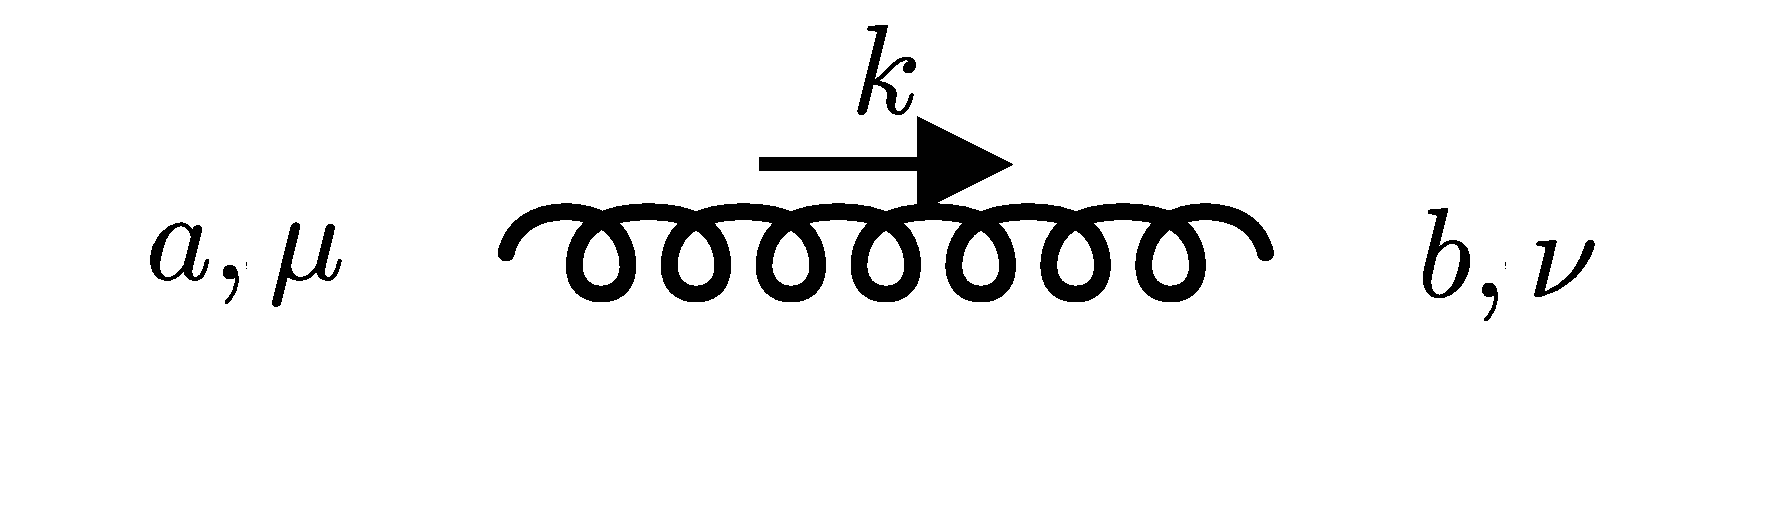
\includegraphics[height=1cm]{Images/FeynmanRules/gluon_propagator.pdf}}} &= i \frac{\delta^{ab}}{k^2 + i 0^+} \left[ -g_{\mu \nu} + (1 - \xi) \frac{k_\mu k_\nu}{k^2 + i 0^+} \right] \\
\vcenter{\hbox{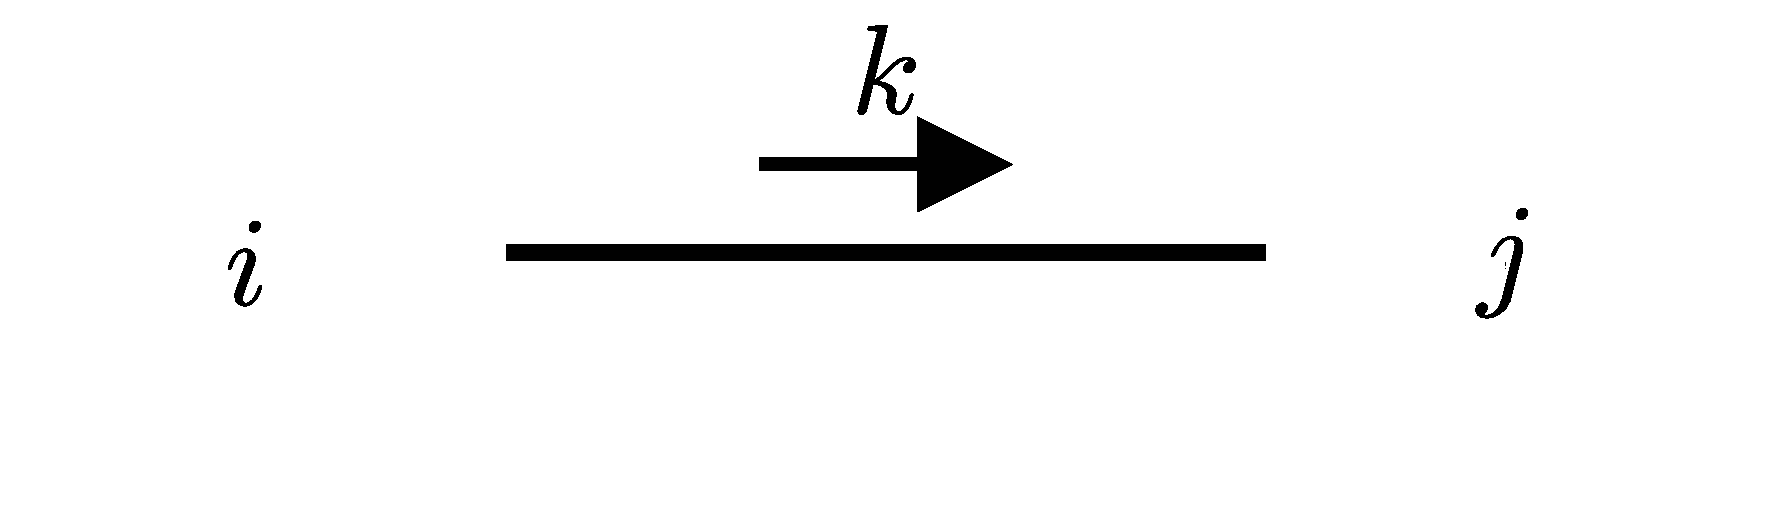
\includegraphics[height=1cm]{Images/FeynmanRules/fermion_propagator.pdf}}} &= i \delta_{ij}\frac{\slashed{k} + m}{k^2 - m^2 + i 0^+}\\
\vcenter{\hbox{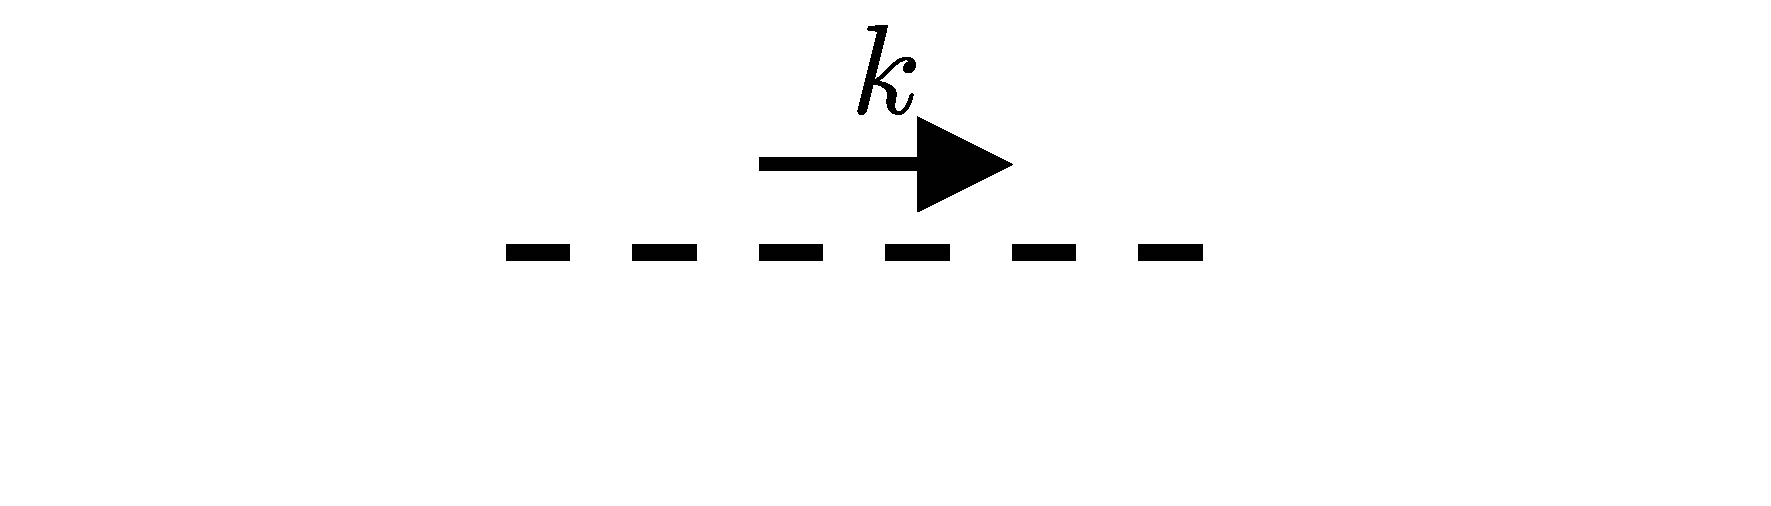
\includegraphics[height=1cm]{Images/FeynmanRules/Higgs_propagator.pdf}}} &= i \frac{1}{k^2 - m_H^2 + i0^+} \\
\vcenter{\hbox{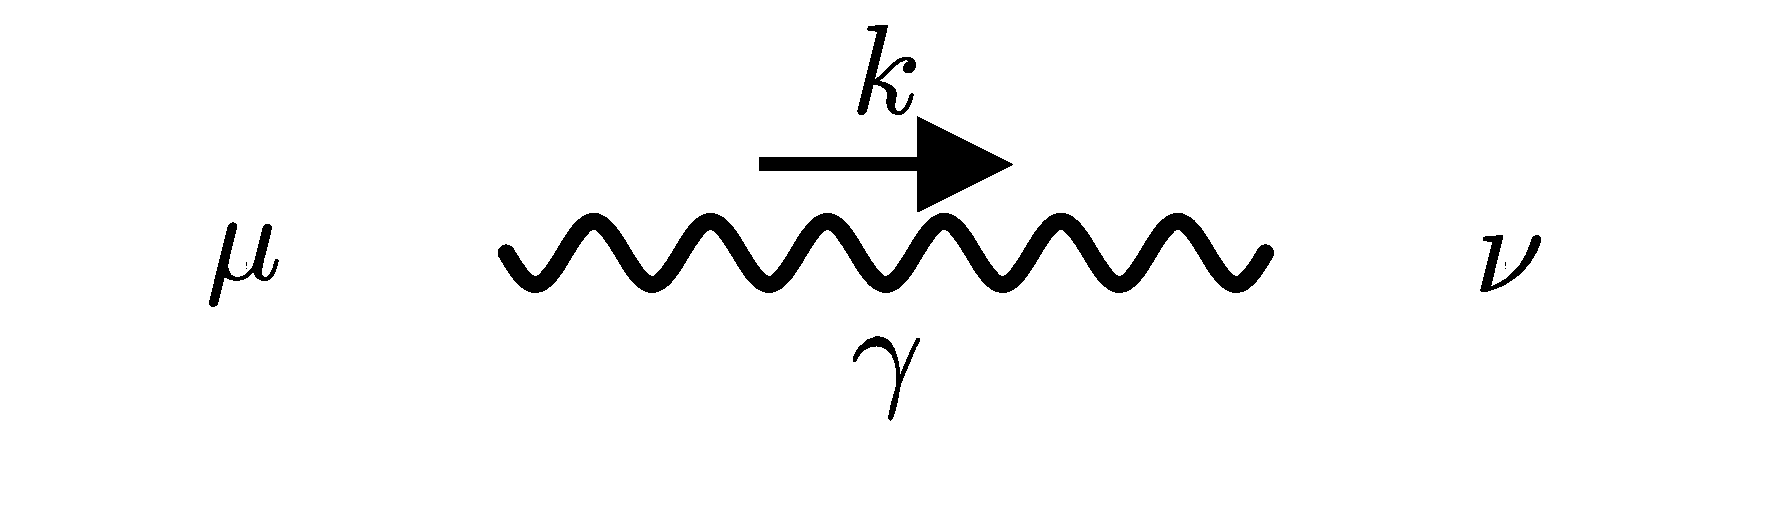
\includegraphics[height=1cm]{Images/FeynmanRules/photon_propagator.pdf}}} &= i \frac{-g_{\mu \nu}}{k^2 + i0^+} \\
\vcenter{\hbox{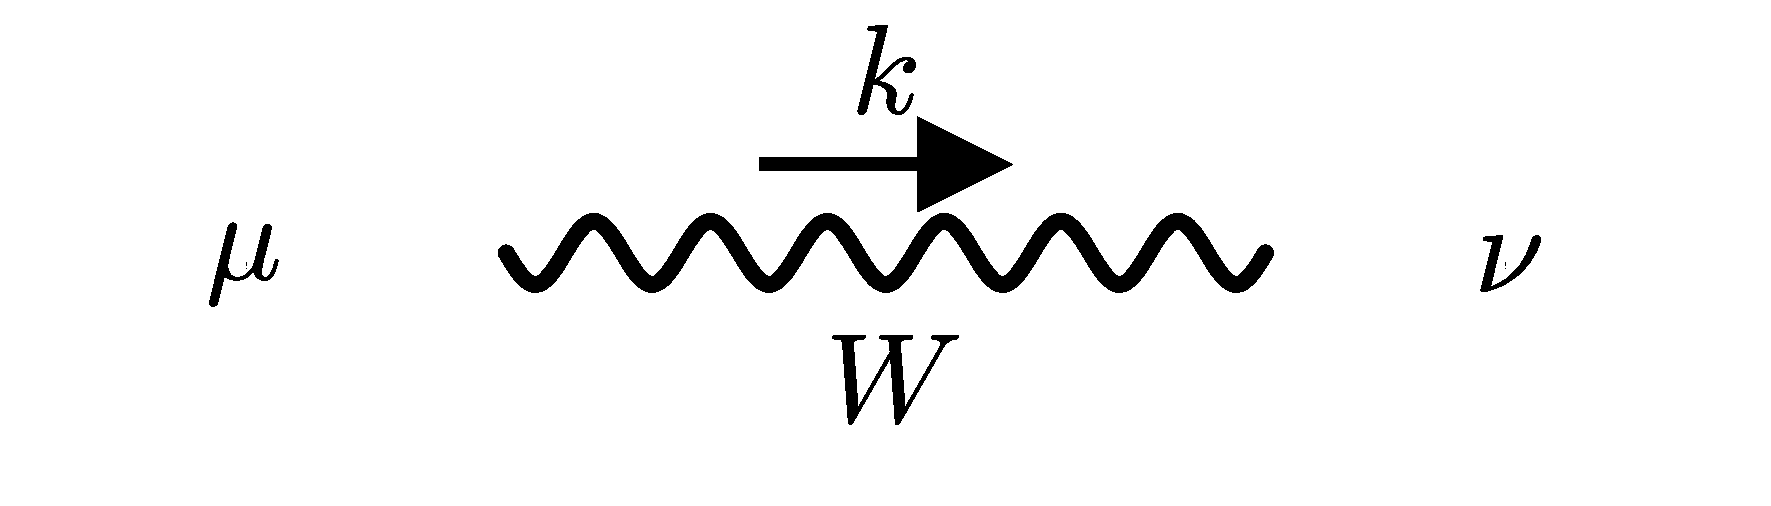
\includegraphics[height=1cm]{Images/FeynmanRules/W_propagator.pdf}}} &= i \frac{1}{k^2 - m_W^2 + i0^+} \left(-g_{\mu\nu} + \frac{k_\mu k_\nu}{m_W^2 + i0^+} \right) \\
\vcenter{\hbox{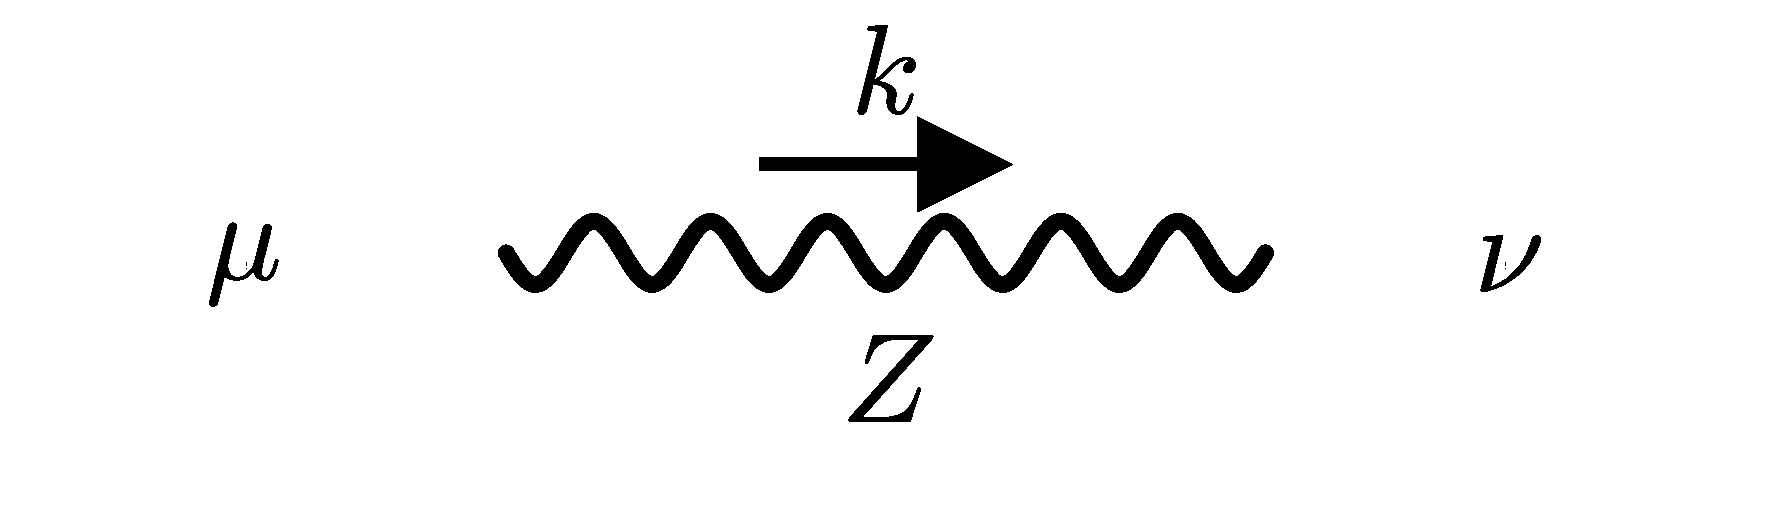
\includegraphics[height=1cm]{Images/FeynmanRules/Z_propagator.pdf}}} &= i \frac{1}{k^2 - m_Z^2 + i0^+} \left(-g_{\mu\nu} + \frac{k_\mu k_\nu}{m_Z^2 + i0^+} \right) \\
\vcenter{\hbox{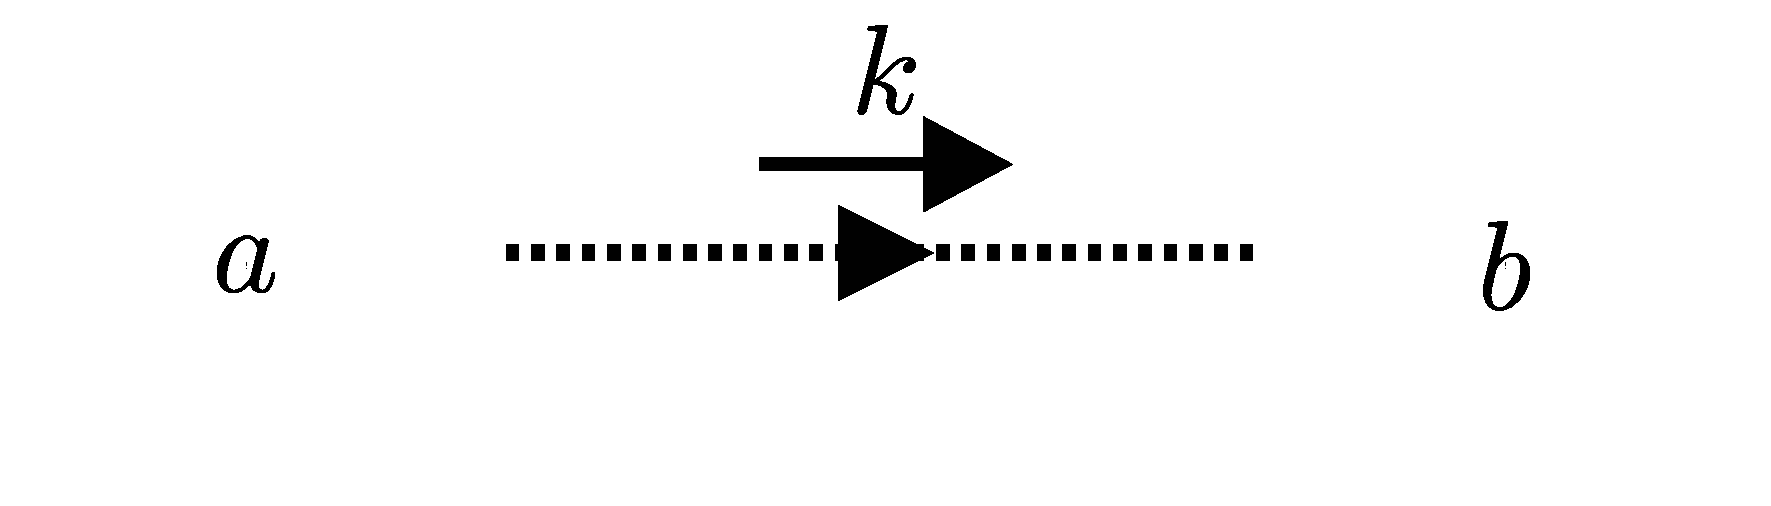
\includegraphics[height=1cm]{Images/FeynmanRules/ghost_propagator.pdf}}} &= i \frac{\delta^{ab}}{k^2 + i 0^+}\\
\end{split}
\end{equation*}

\textbf{Fermion--Gauge-Boson Vertices:}
\begin{alignat*}{3}
&\vcenter{\hbox{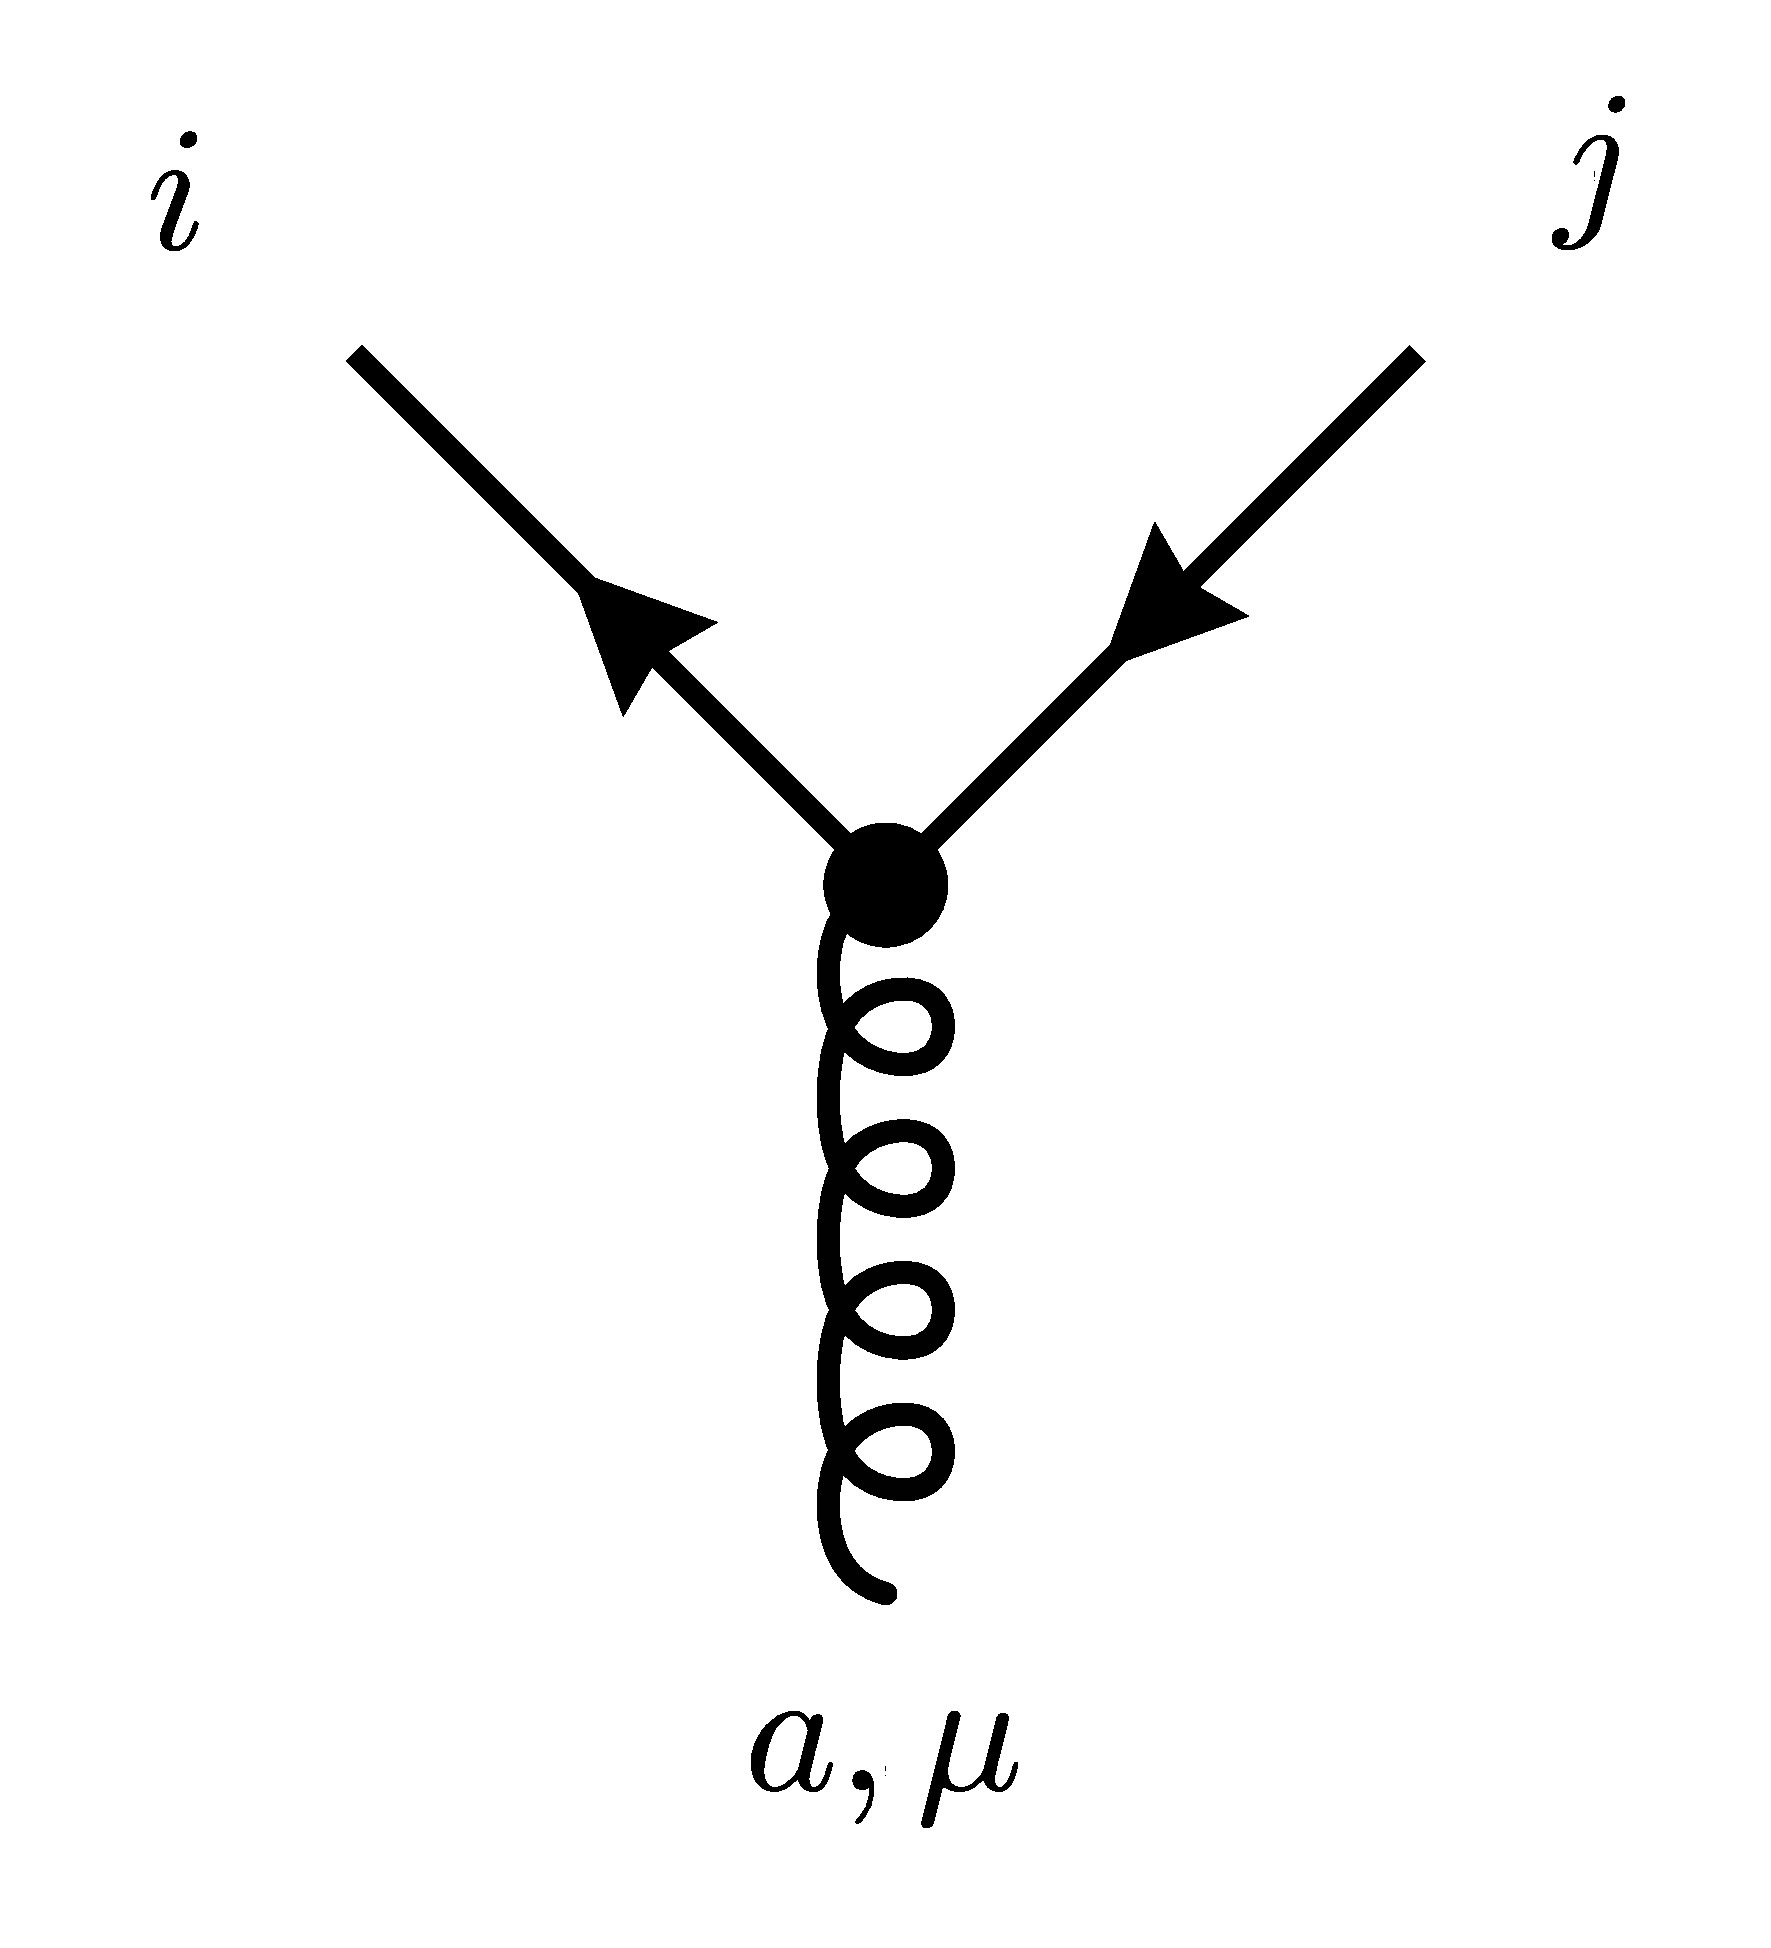
\includegraphics[width=3cm]{Images/FeynmanRules/gluon_fermion_vertex.pdf}}} = i g \gamma^\mu T^a_{ij} \quad
&&\vcenter{\hbox{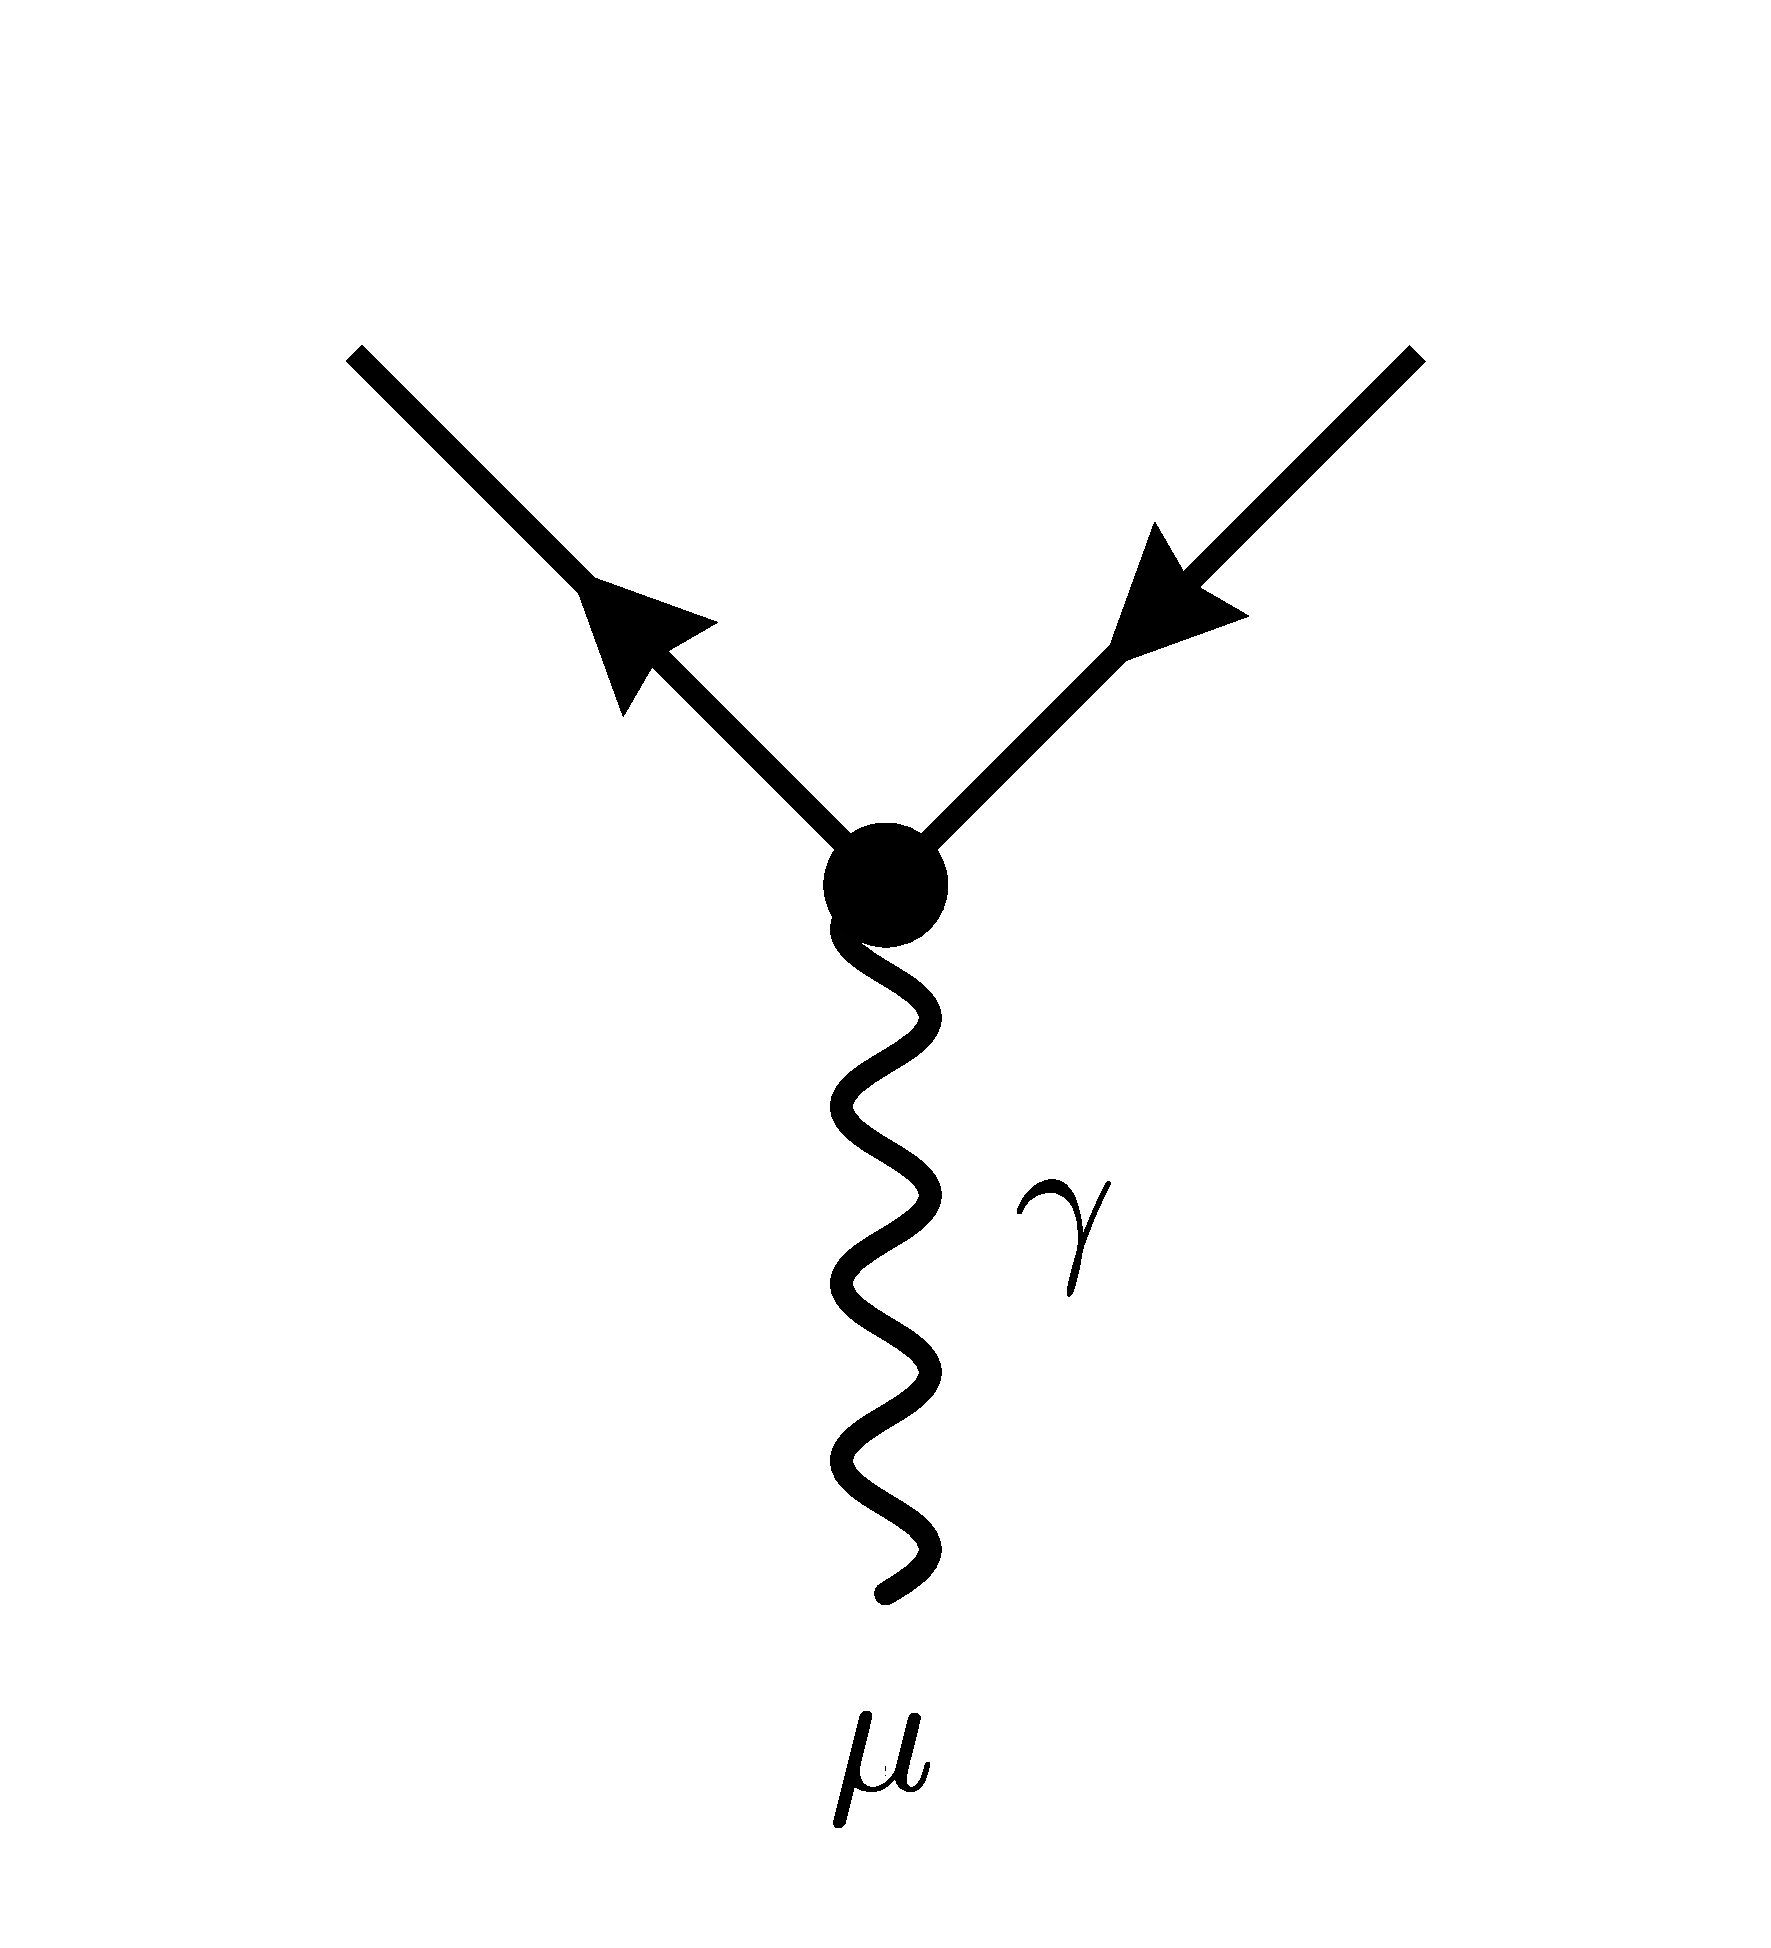
\includegraphics[width=3cm]{Images/FeynmanRules/photon_fermion_vertex.pdf}}}= -i e \gamma^\mu Q   \\
%
&\vcenter{\hbox{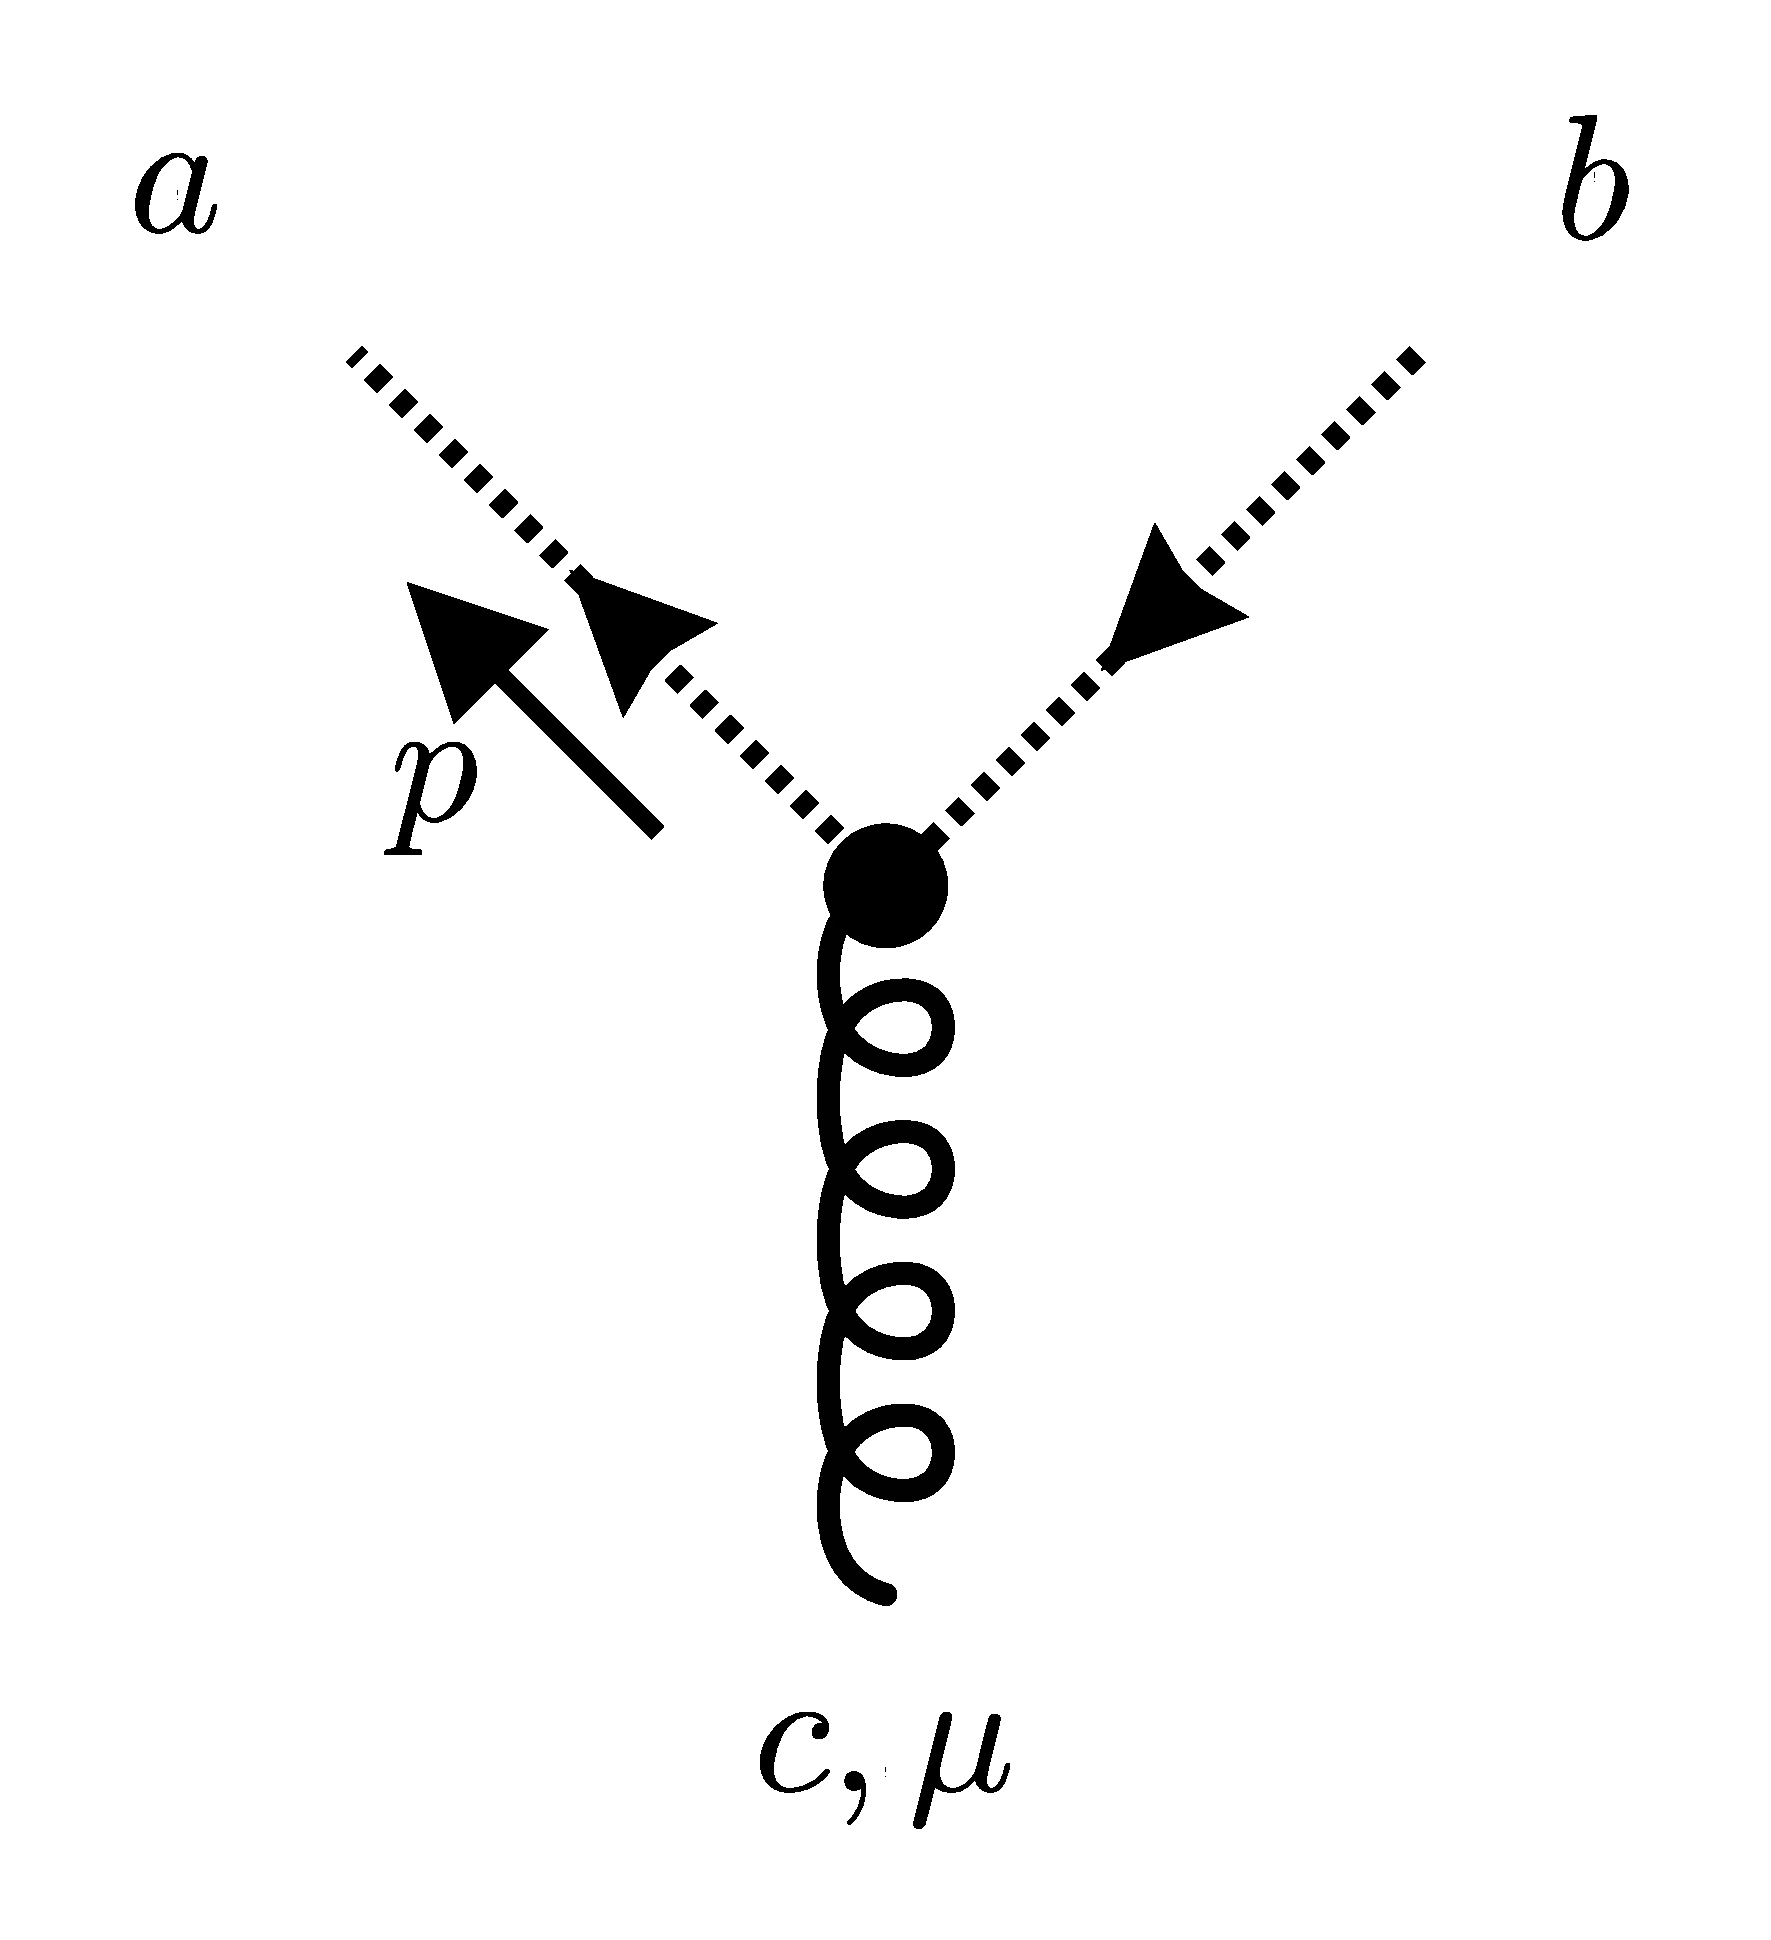
\includegraphics[width=3cm]{Images/FeynmanRules/gluon_ghost_vertex.pdf}}} = g f^{abc} p^\mu  \quad
&&\vcenter{\hbox{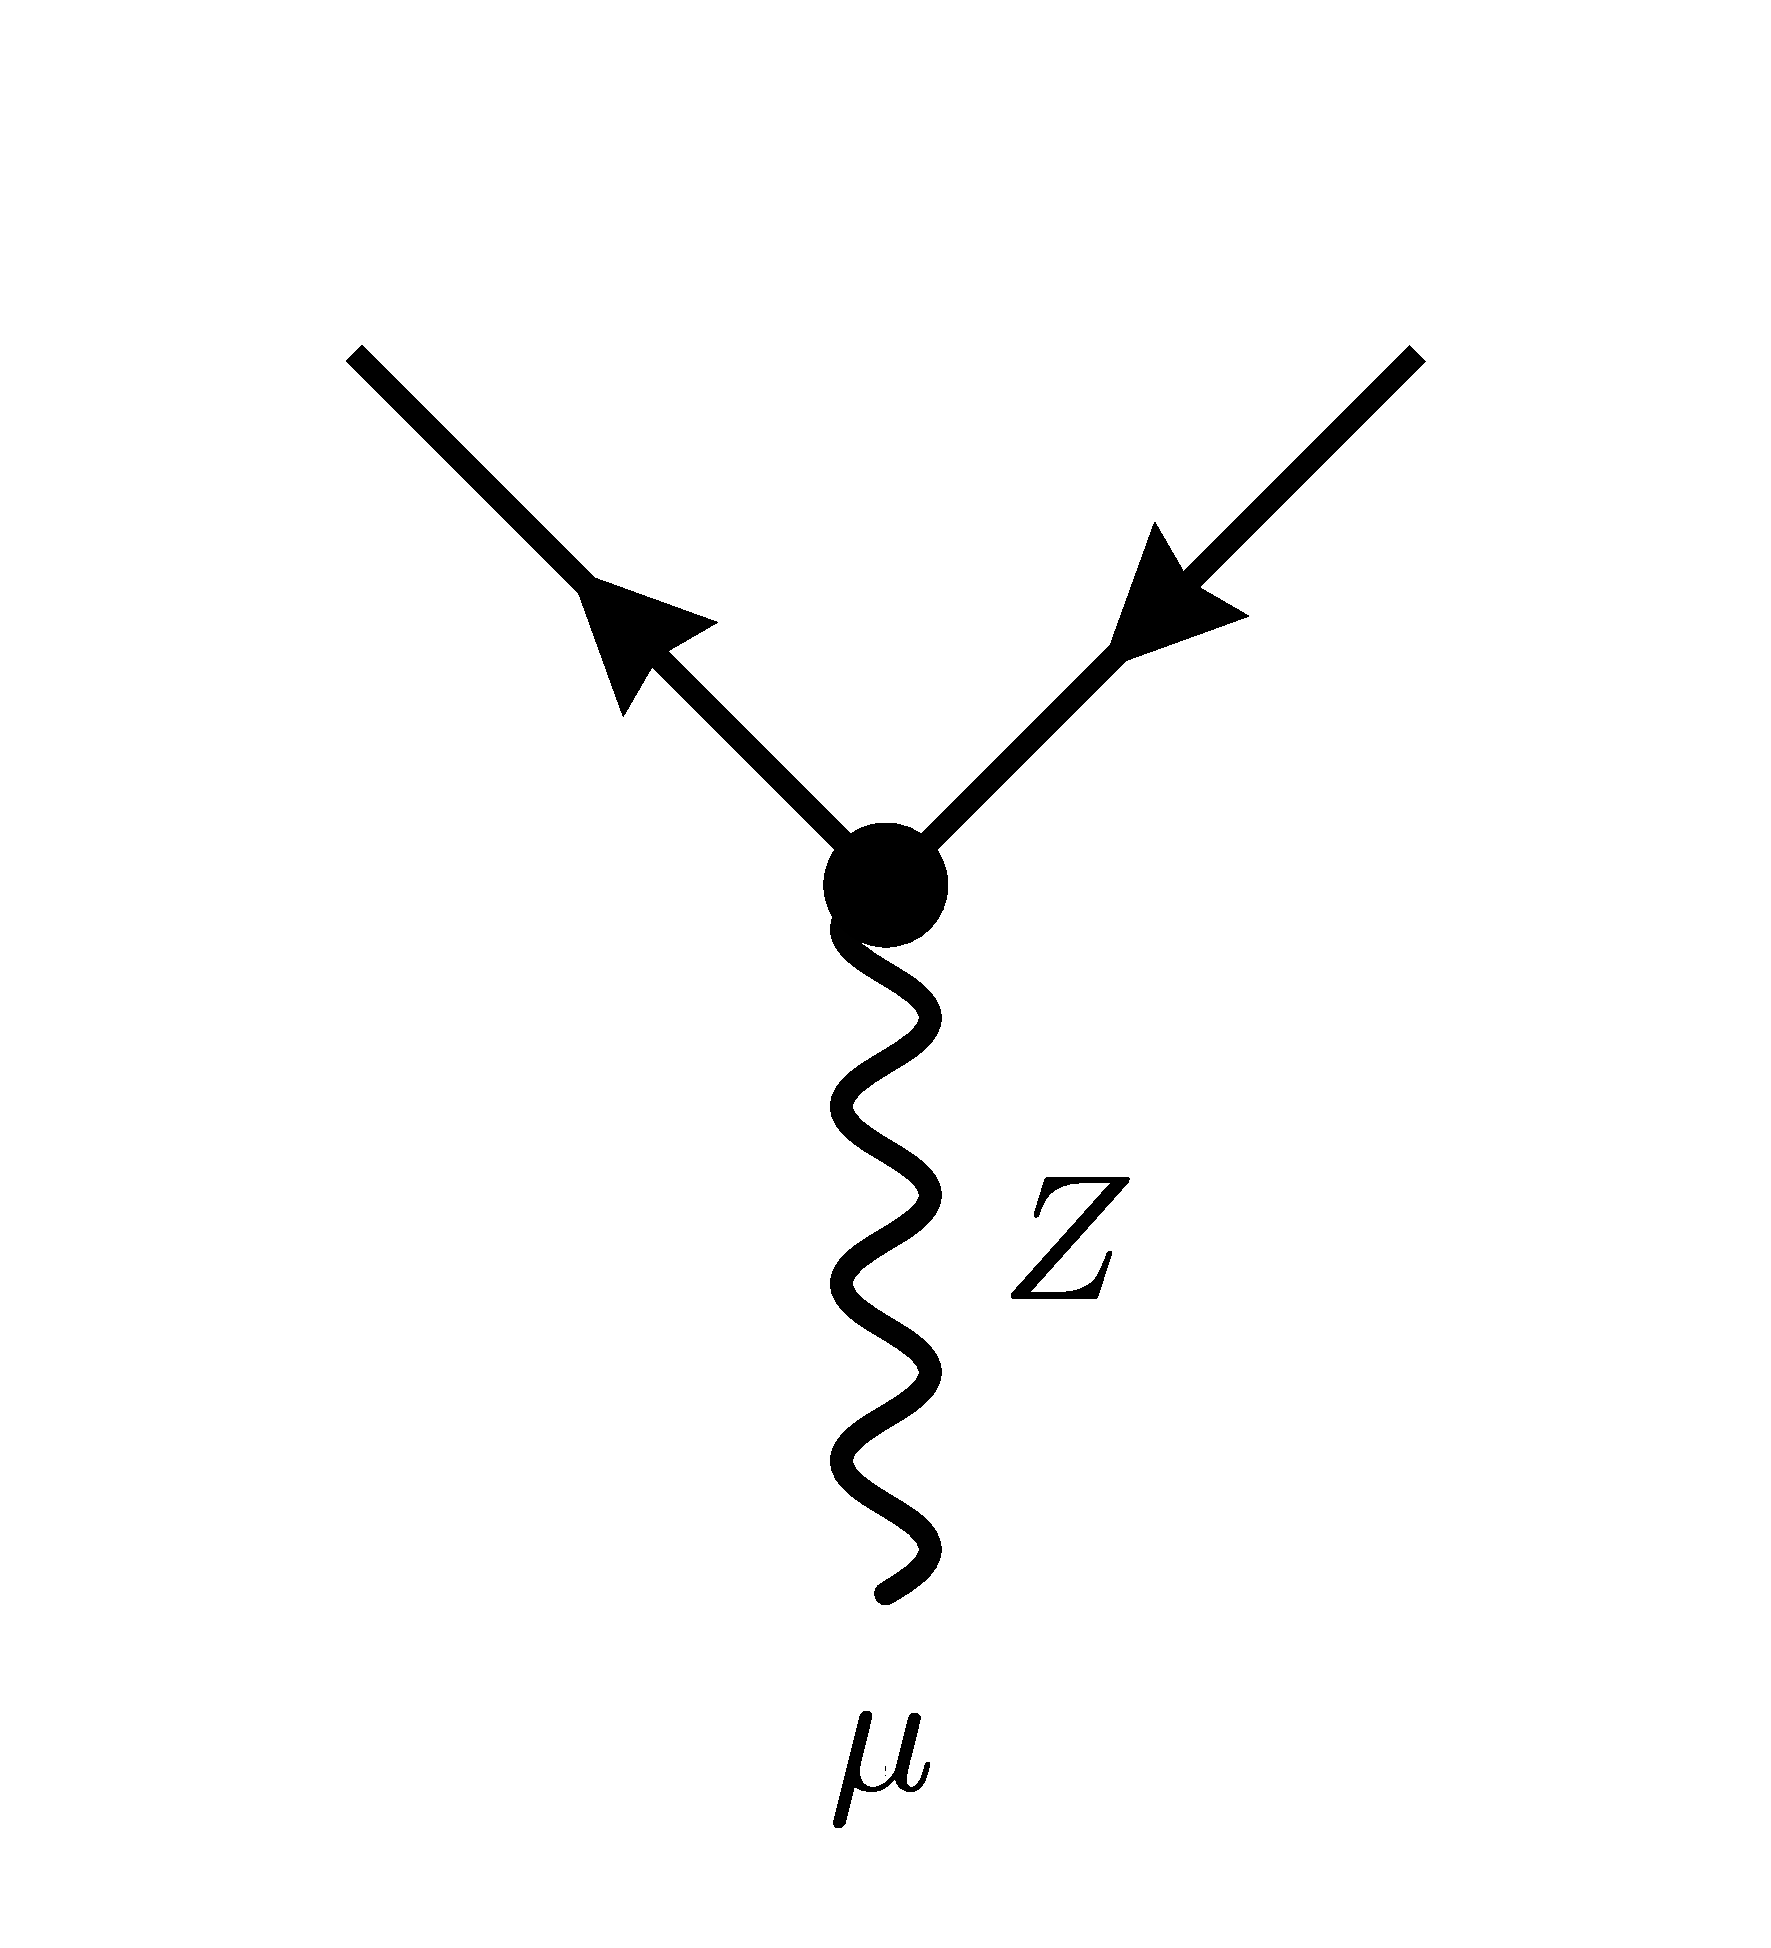
\includegraphics[width=3cm]{Images/FeynmanRules/Z_fermion_vertex.pdf}}} \subalign{=\ &i \frac{e}{\sin  \theta_W \cos\theta_W} \gamma^\mu \\ &\ \times \left(I^3 P_L - Q \sin^2 \theta_W \right)}  \\
%
&\vcenter{\hbox{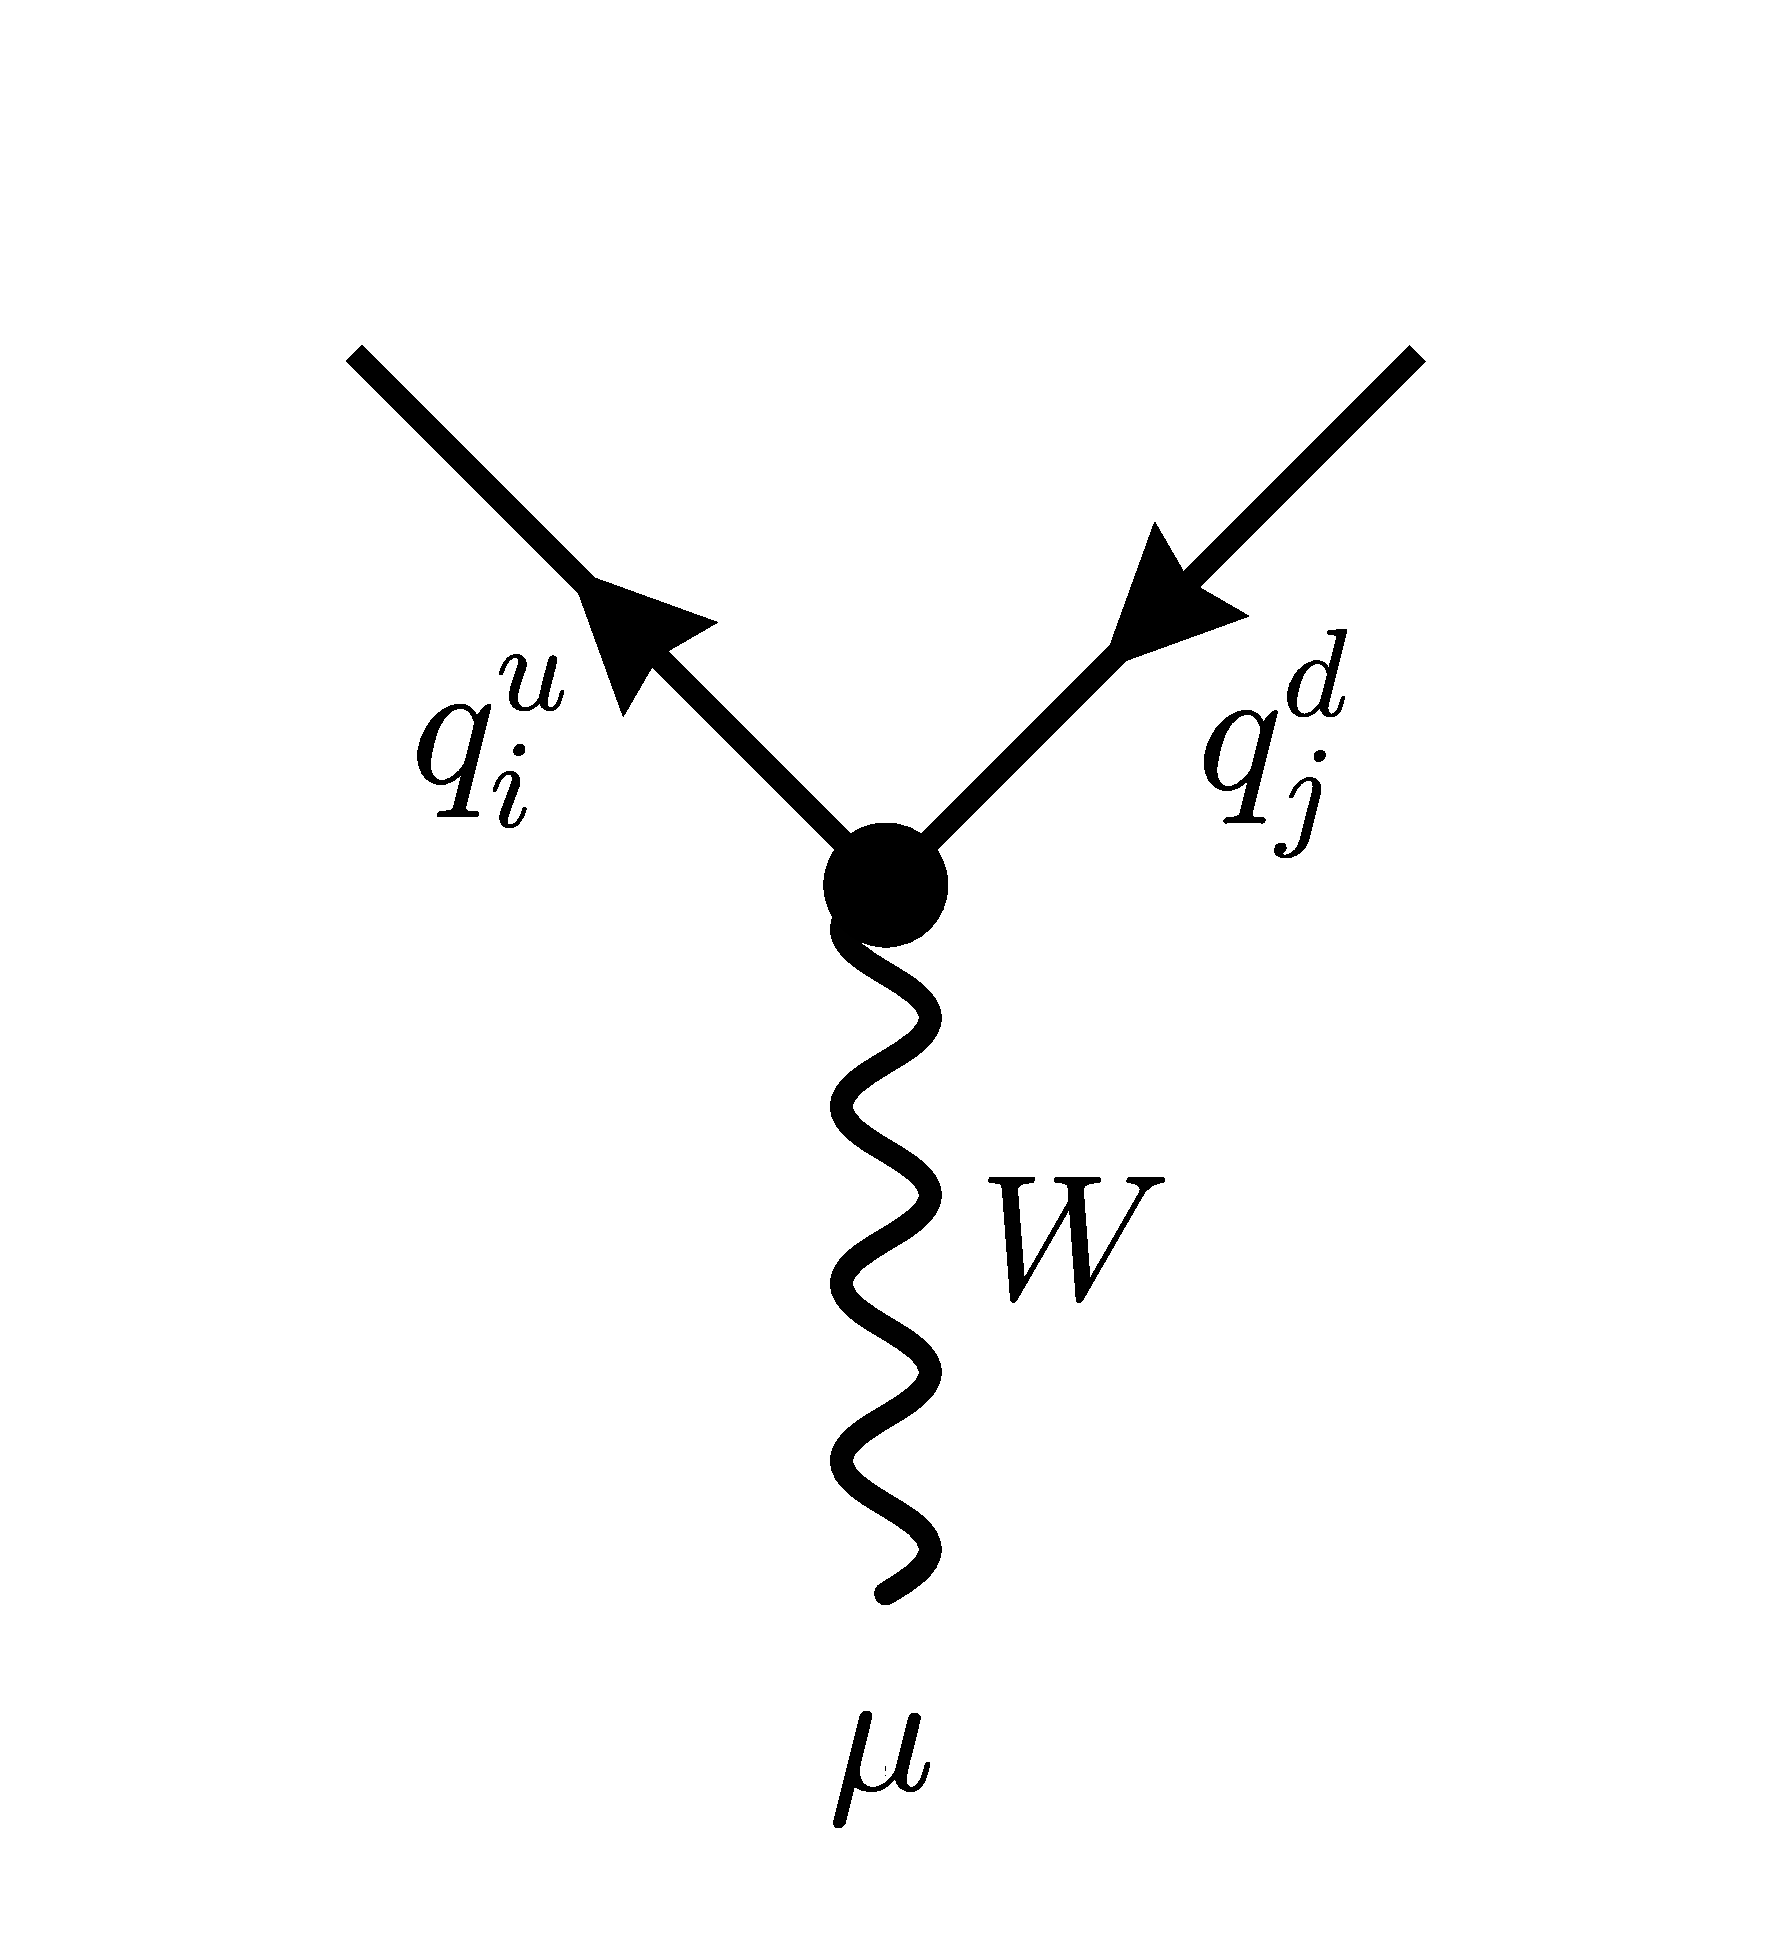
\includegraphics[width=3cm]{Images/FeynmanRules/W_fermion_vertex.pdf}}} = i \frac{e(V_{\text{CKM}})_{ij}}{\sqrt{2} \sin \theta_W} \gamma^\mu P_L  \quad
&&\vcenter{\hbox{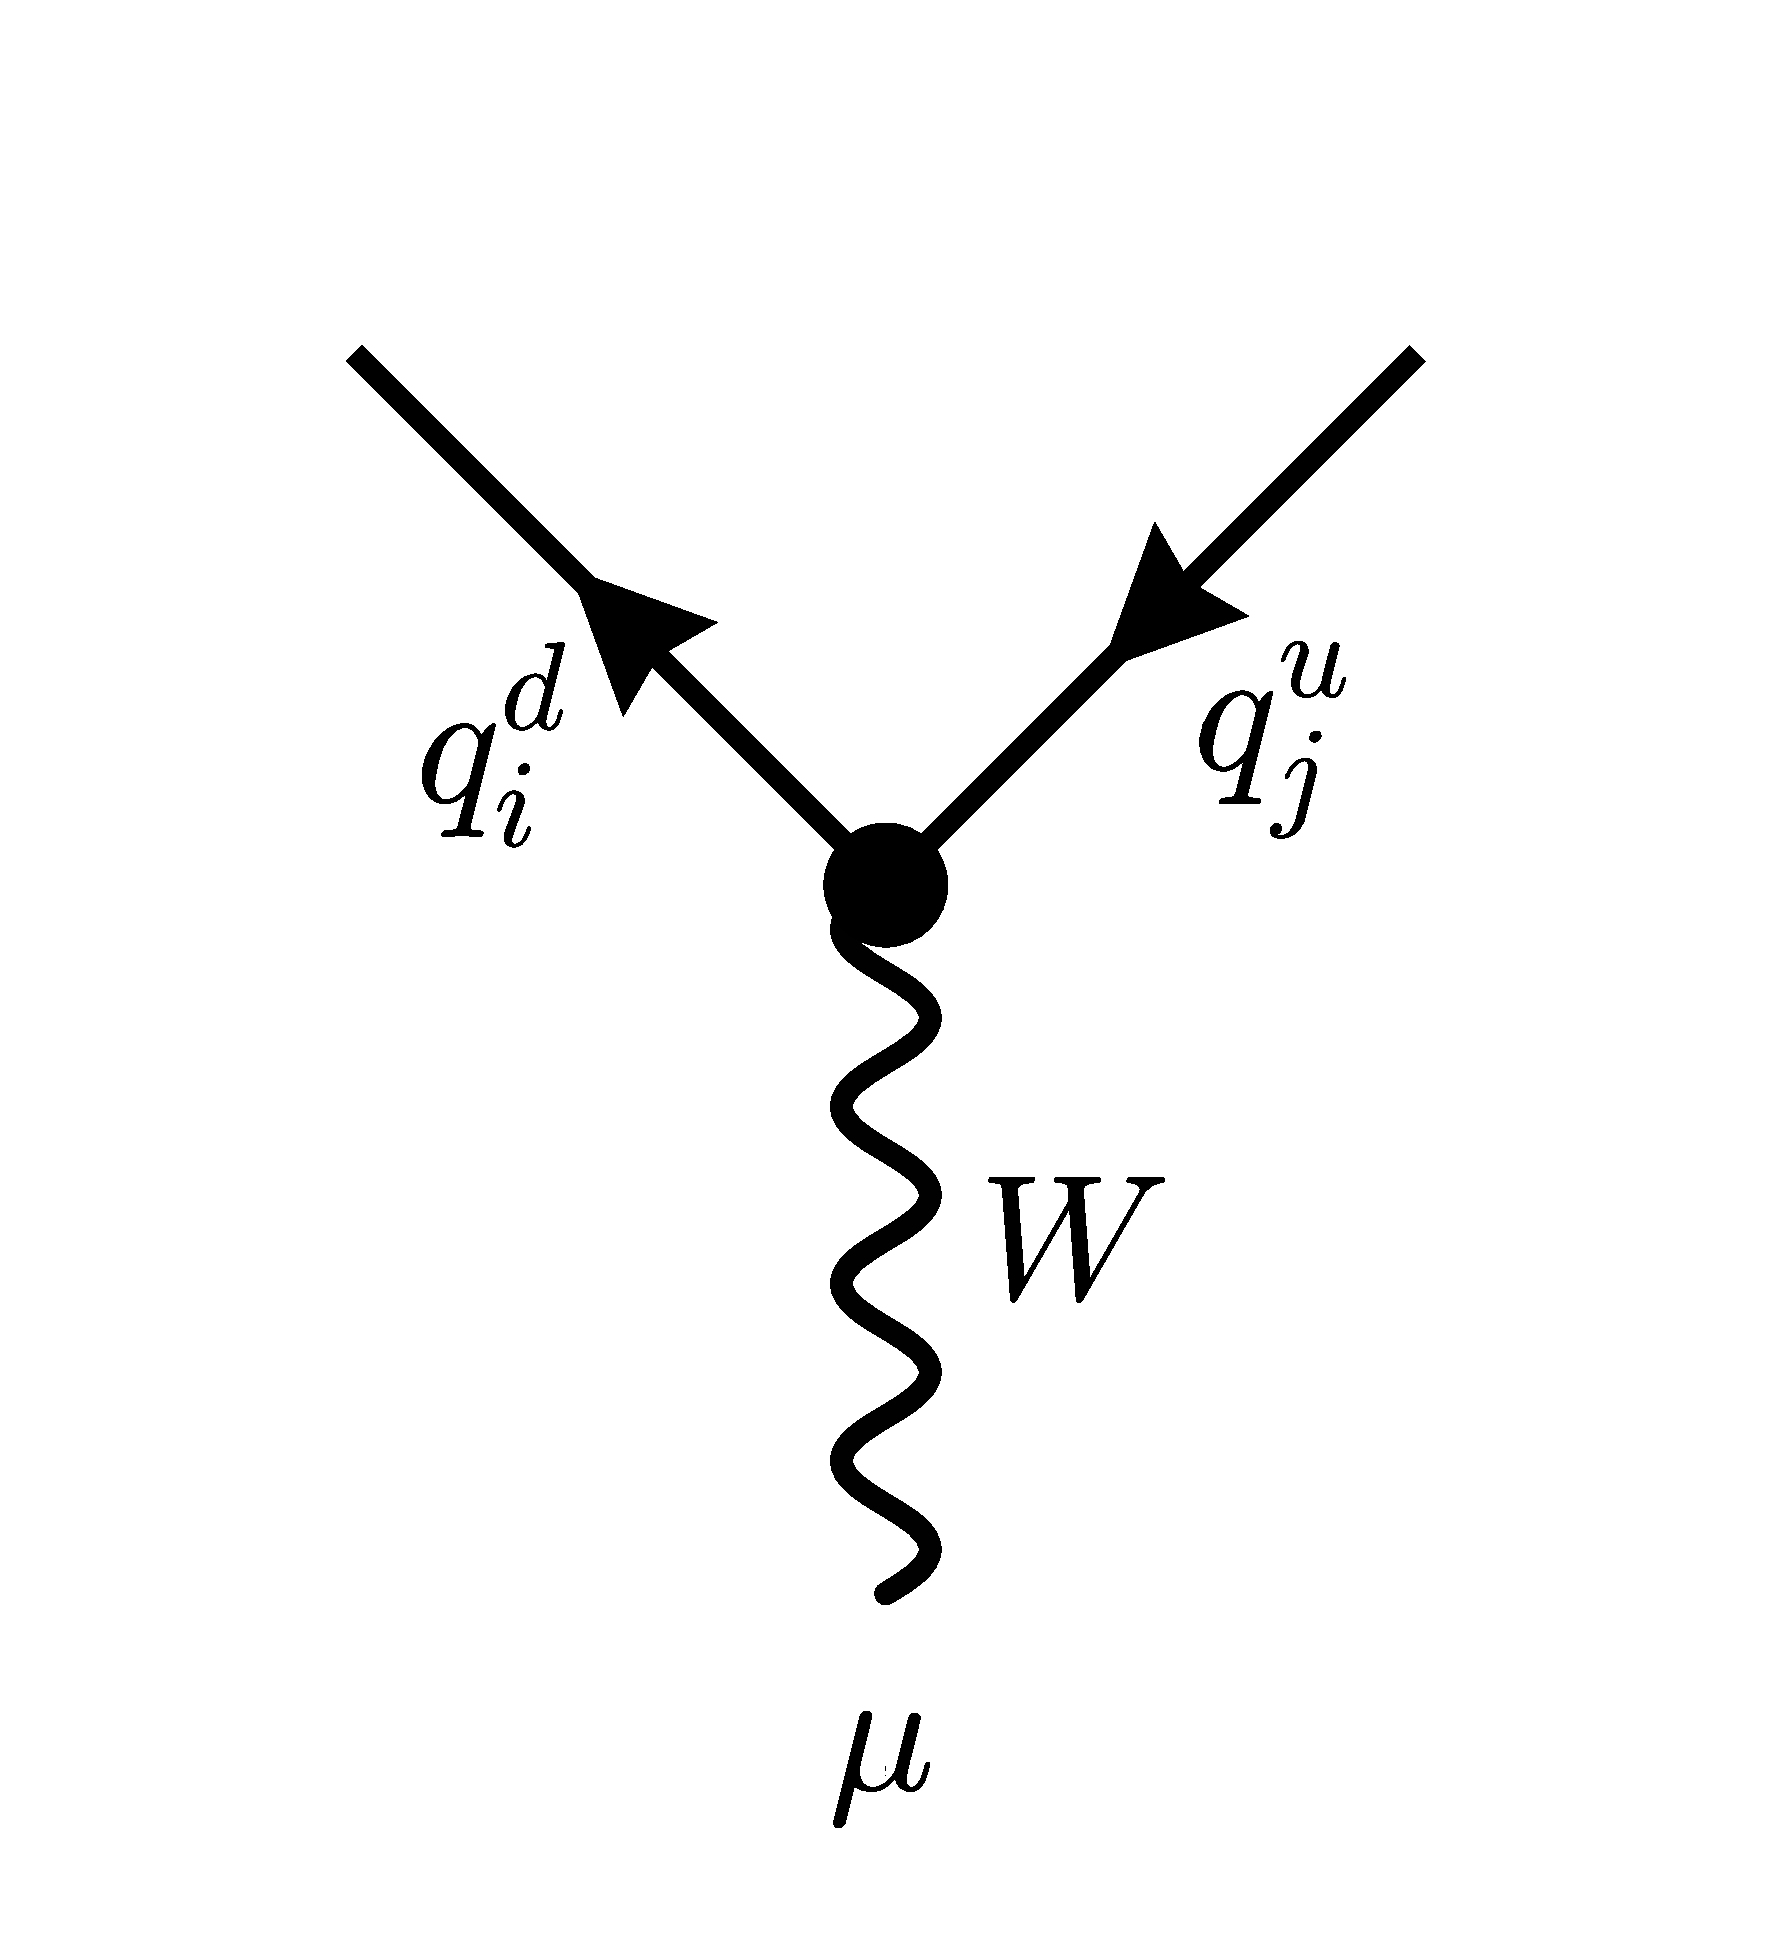
\includegraphics[width=3cm]{Images/FeynmanRules/W_fermion_vertex_2.pdf}}} = i \frac{e(V_{\text{CKM}})_{ji}^*}{\sqrt{2} \sin \theta_W} \gamma^\mu P_L
\end{alignat*}

\textbf{Gauge-Boson Self Interactions:}
\begin{alignat*}{3}
\vcenter{\hbox{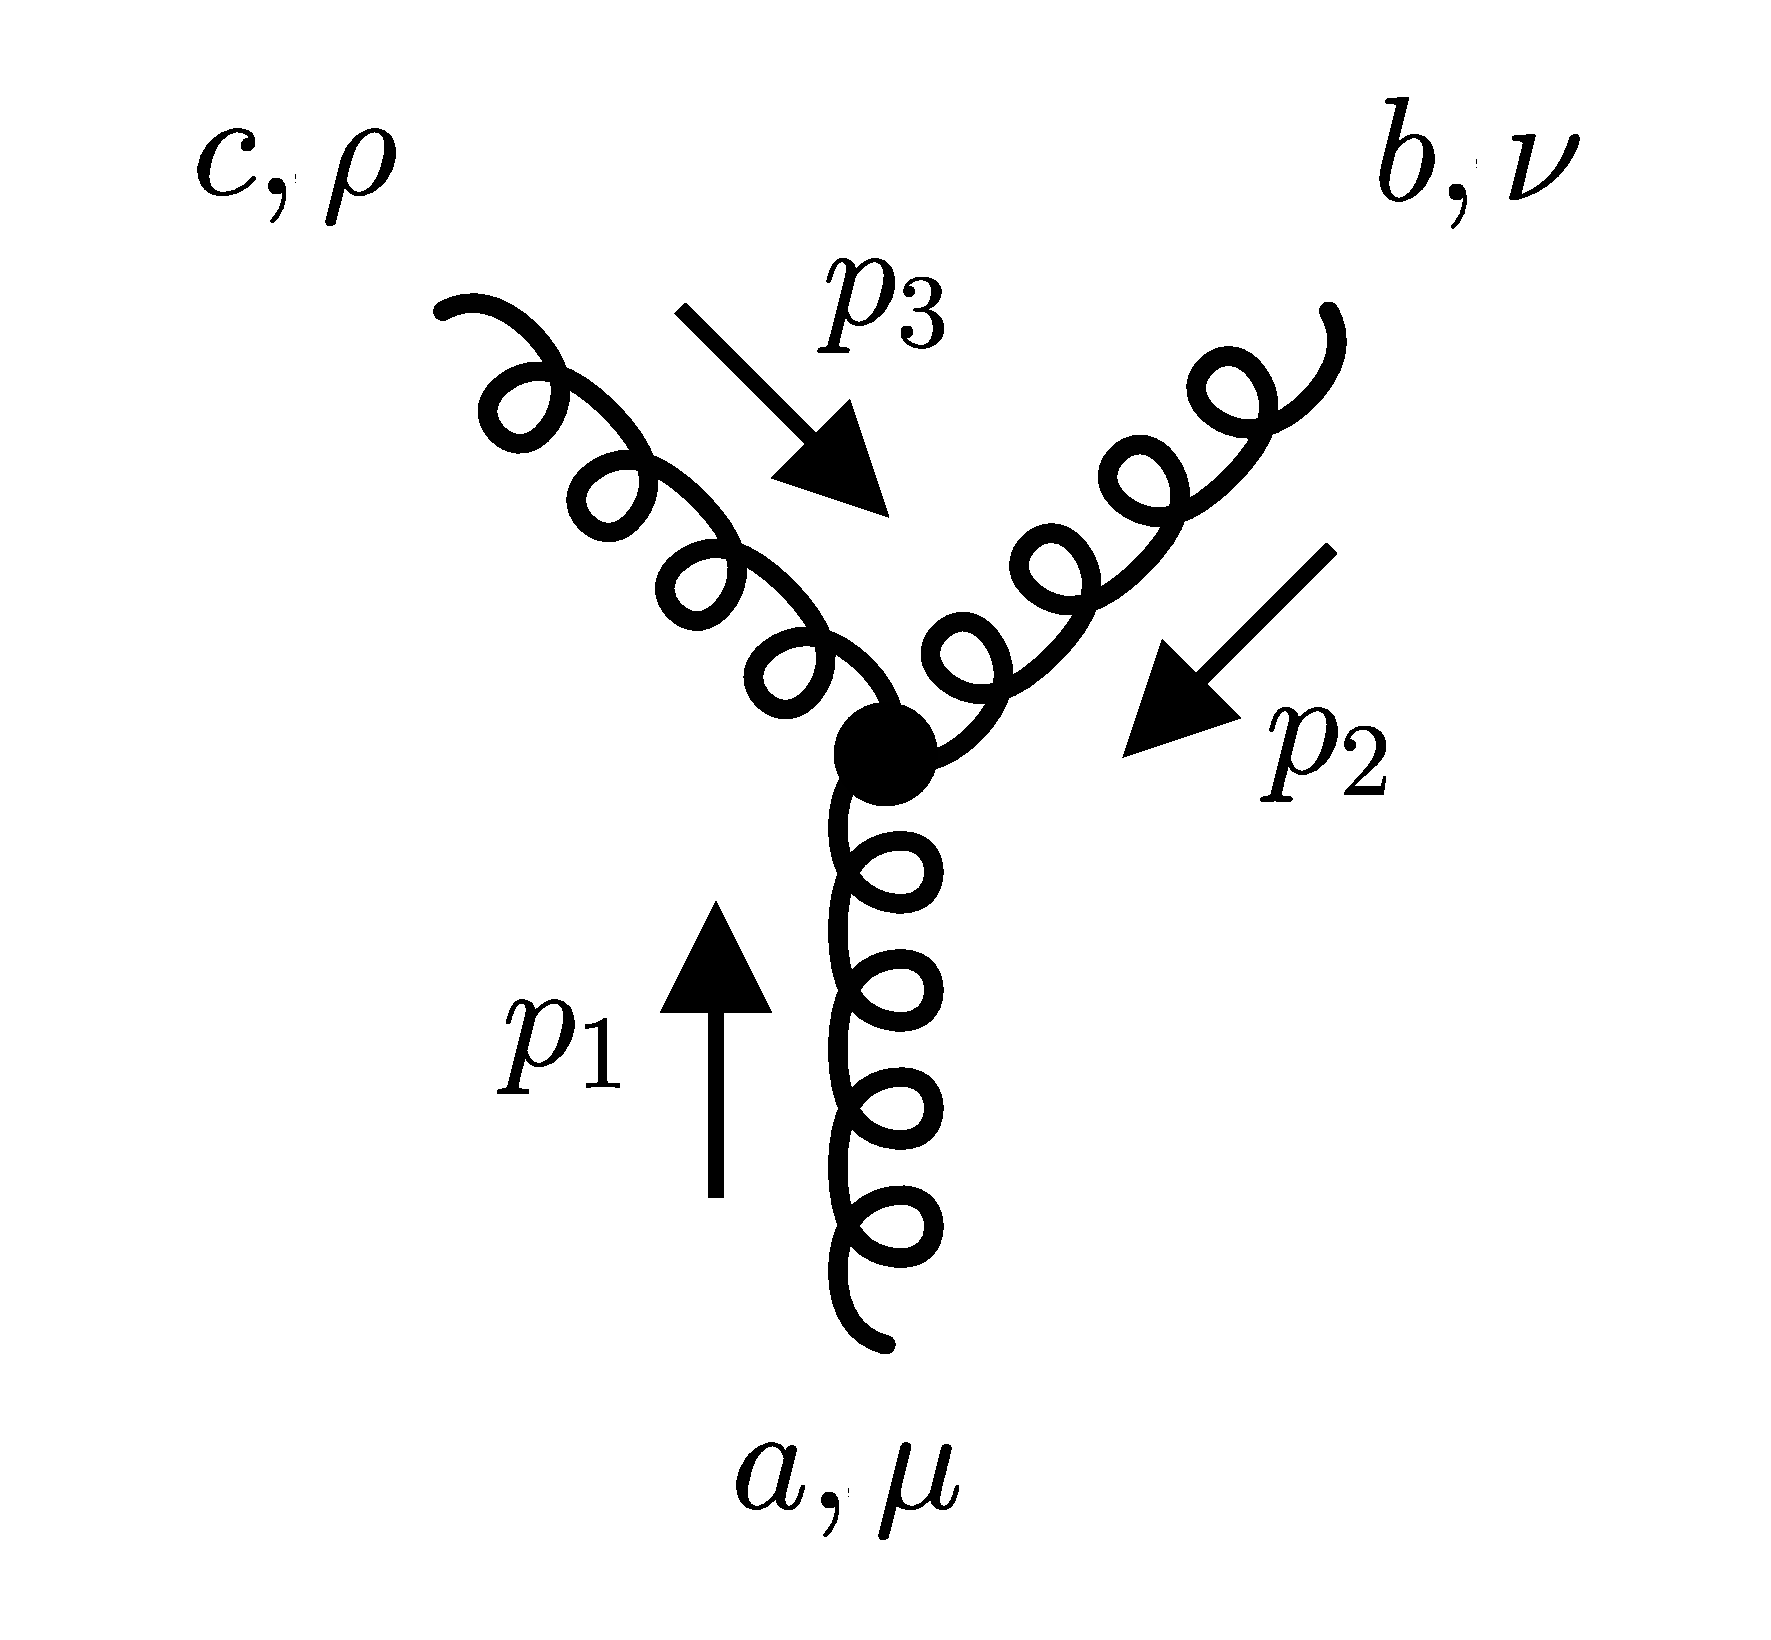
\includegraphics[width=3cm]{Images/FeynmanRules/triple_gluon_vertex.pdf}}} &  \subalign{=g f^{abc} ( &(p_1^\rho - p_2^\rho) g^{\mu \nu} \\ &+ (p_2^\mu - p_3^\mu) g^{\nu\rho} + (p_3^\nu - p_1^\nu) g^{\rho \mu})} \\
%
\vcenter{\hbox{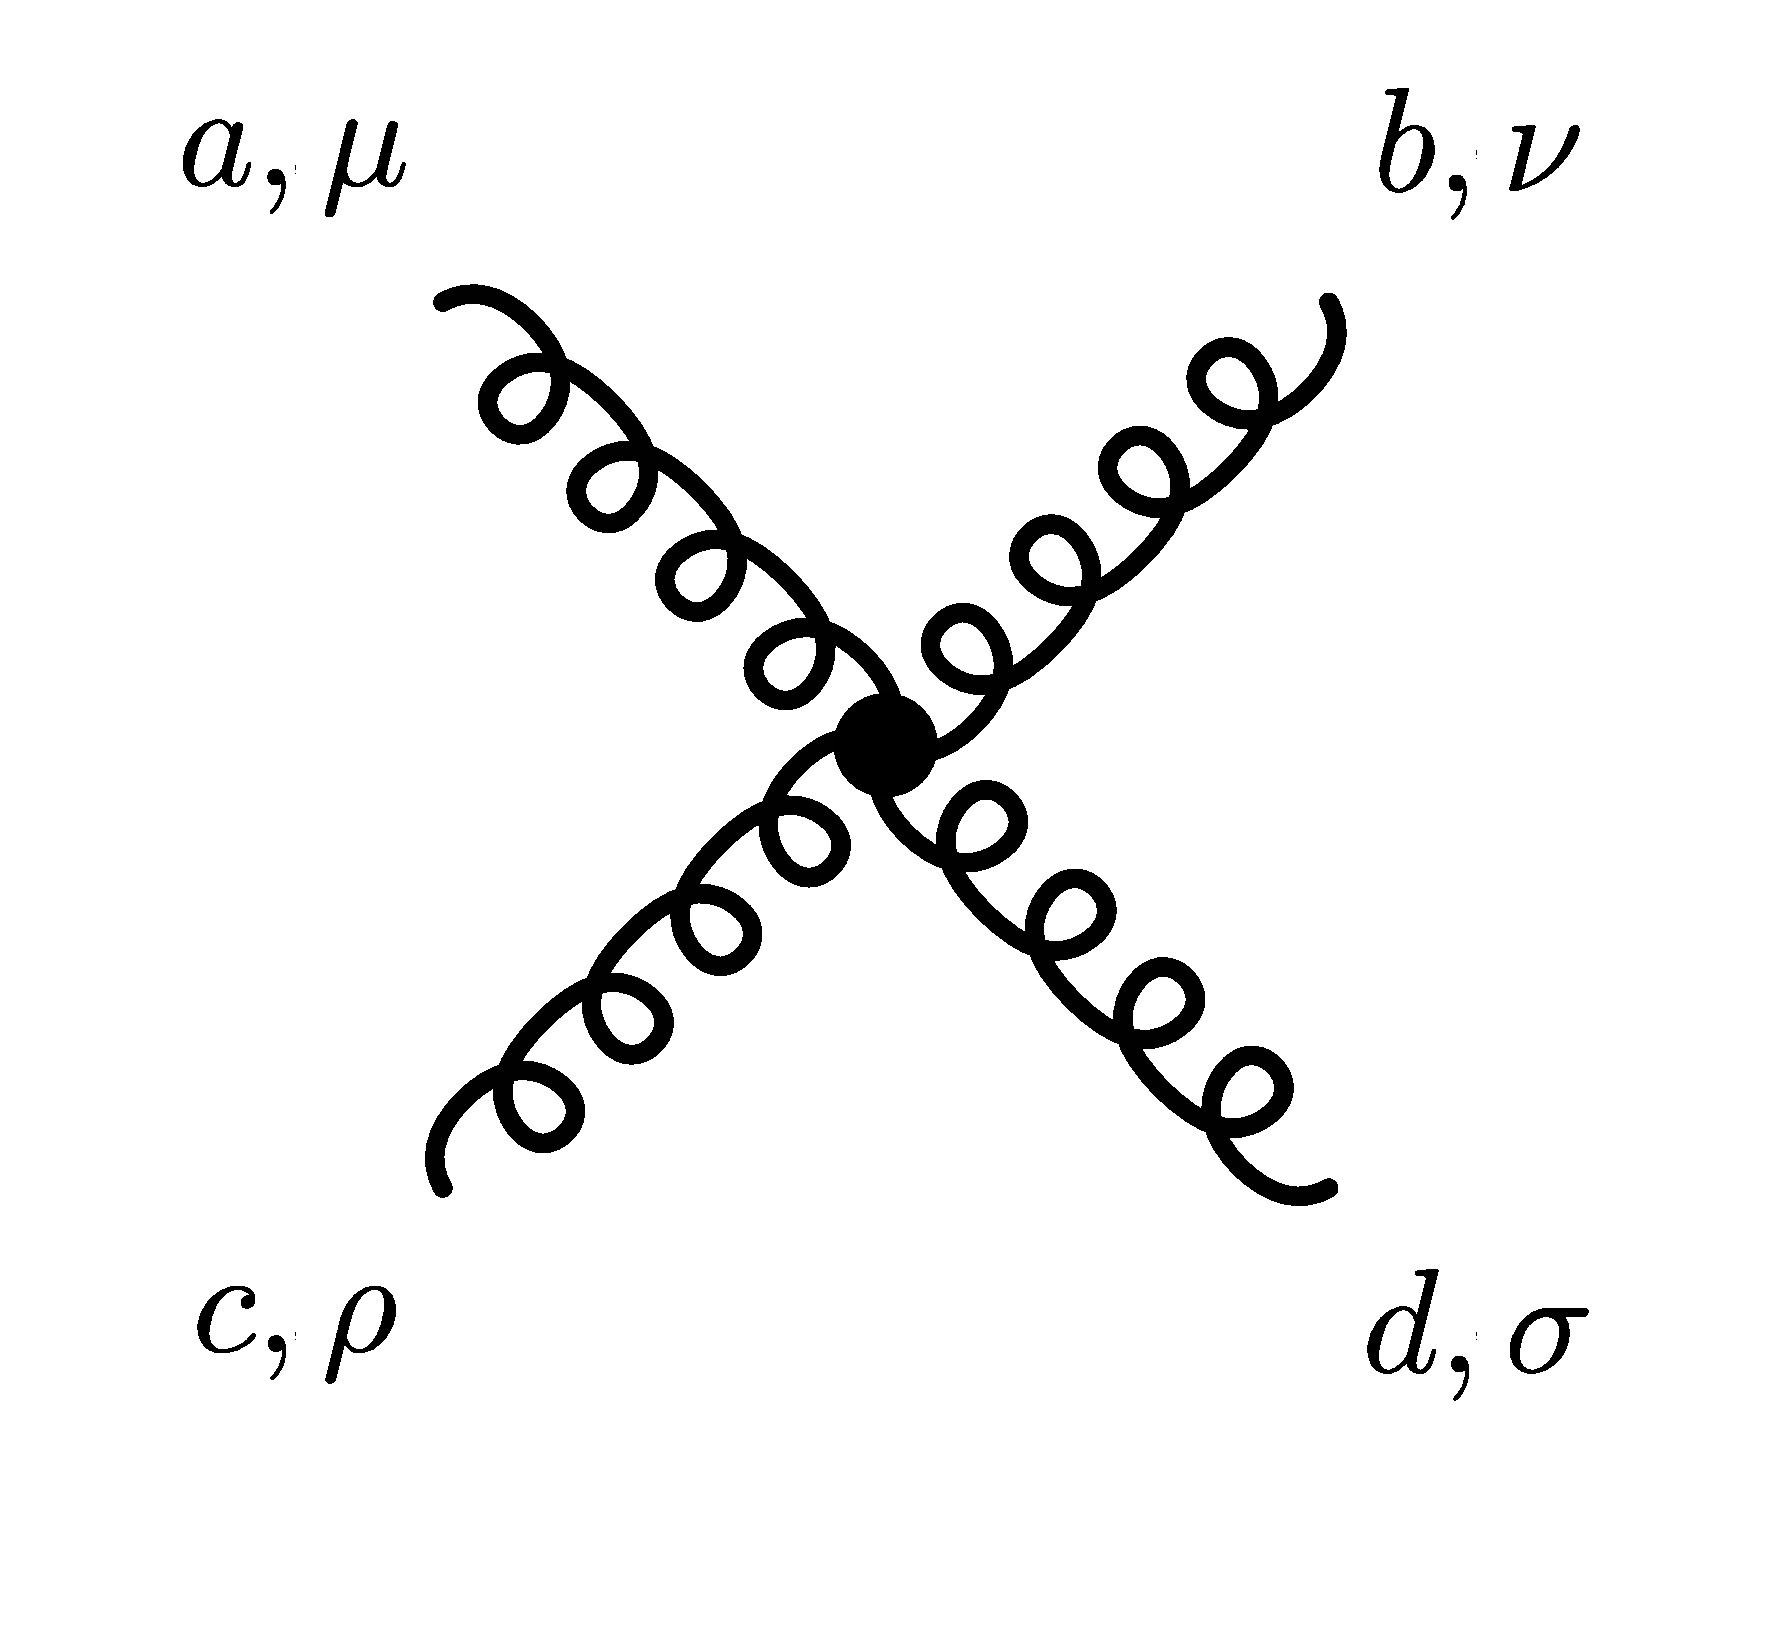
\includegraphics[width=3cm]{Images/FeynmanRules/quadruple_gluon_vertex.pdf}}} & \subalign{=-ig^2 \big ( &f^{abe}f^{cde} (g^{\mu \rho} g^{\nu \sigma} - g^{\mu \sigma} g^{\nu \rho}) \\ +&f^{ace} f^{bde} (g^{\mu \nu} g^{\rho \sigma} - g^{\mu \sigma} g^{\nu \rho}) \\ +&f^{ade}f^{bce} (g^{\mu \nu} g^{\rho \sigma} - g^{\mu \rho} g^{\nu \sigma}) \big )}   \\
%
\vcenter{\hbox{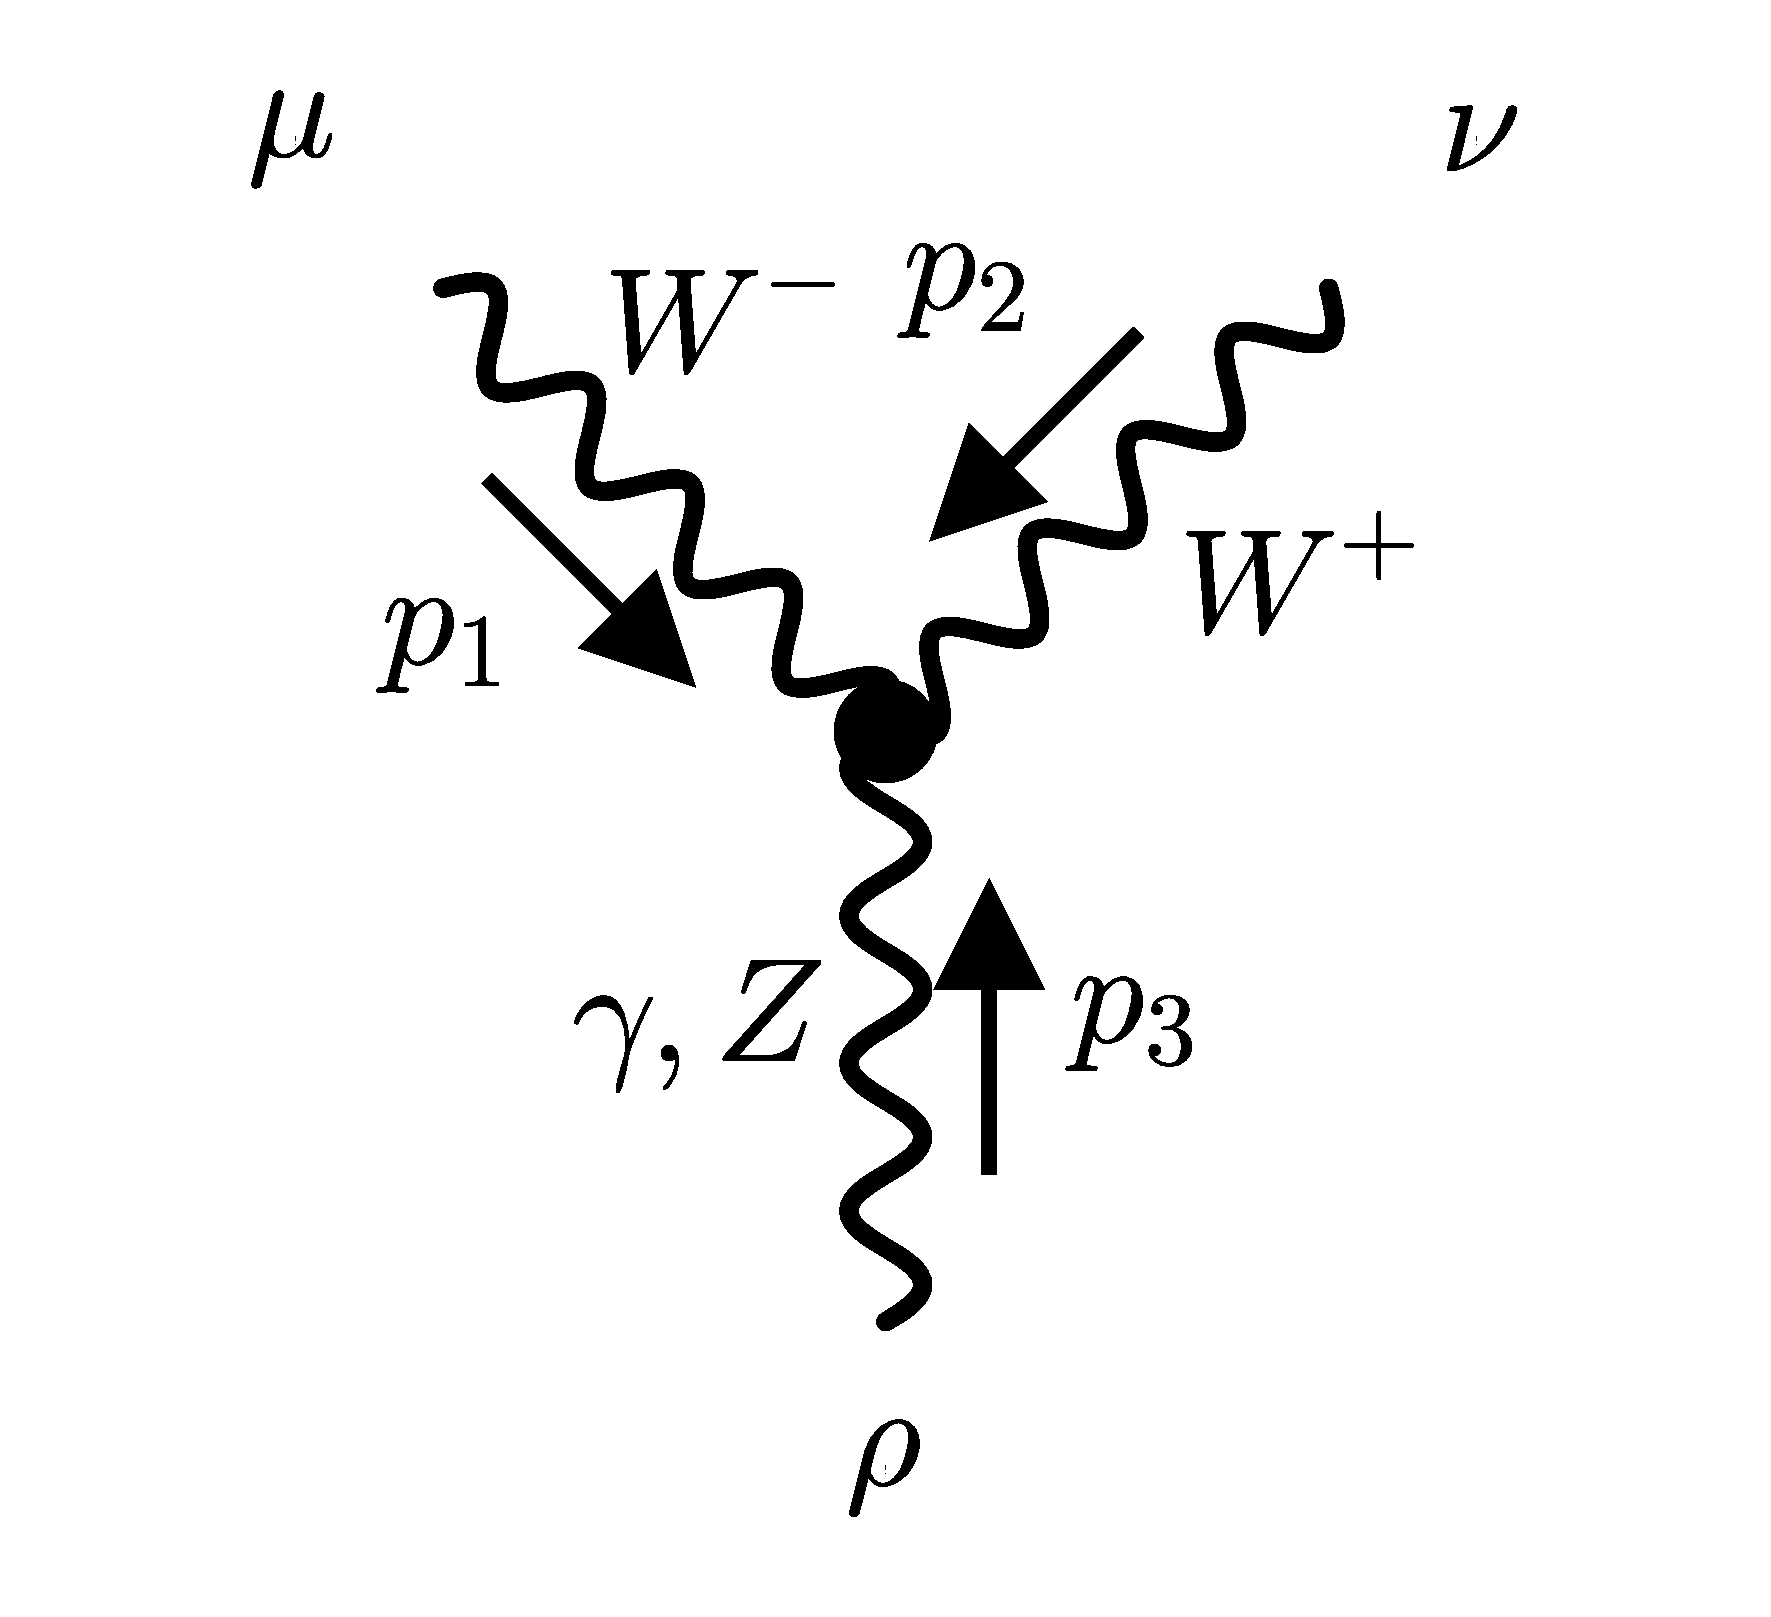
\includegraphics[width=3cm]{Images/FeynmanRules/photon_W_vertex.pdf}}} & \subalign{  = i \frac{e}{\sin\theta_W} ( &(p_1^\rho - p_2^\rho) g^{\mu \nu} + (p_2^\mu - p_3^\mu) g^{\nu \rho} \\ + &(p_3^\nu - p_1^\nu) g^{\rho \mu} ) \times \begin{cases}  -\sin \theta_W \quad &\text{for }\gamma \\ \cos \theta_W \quad &\text{for }Z \end{cases}} \\
%
\vcenter{\hbox{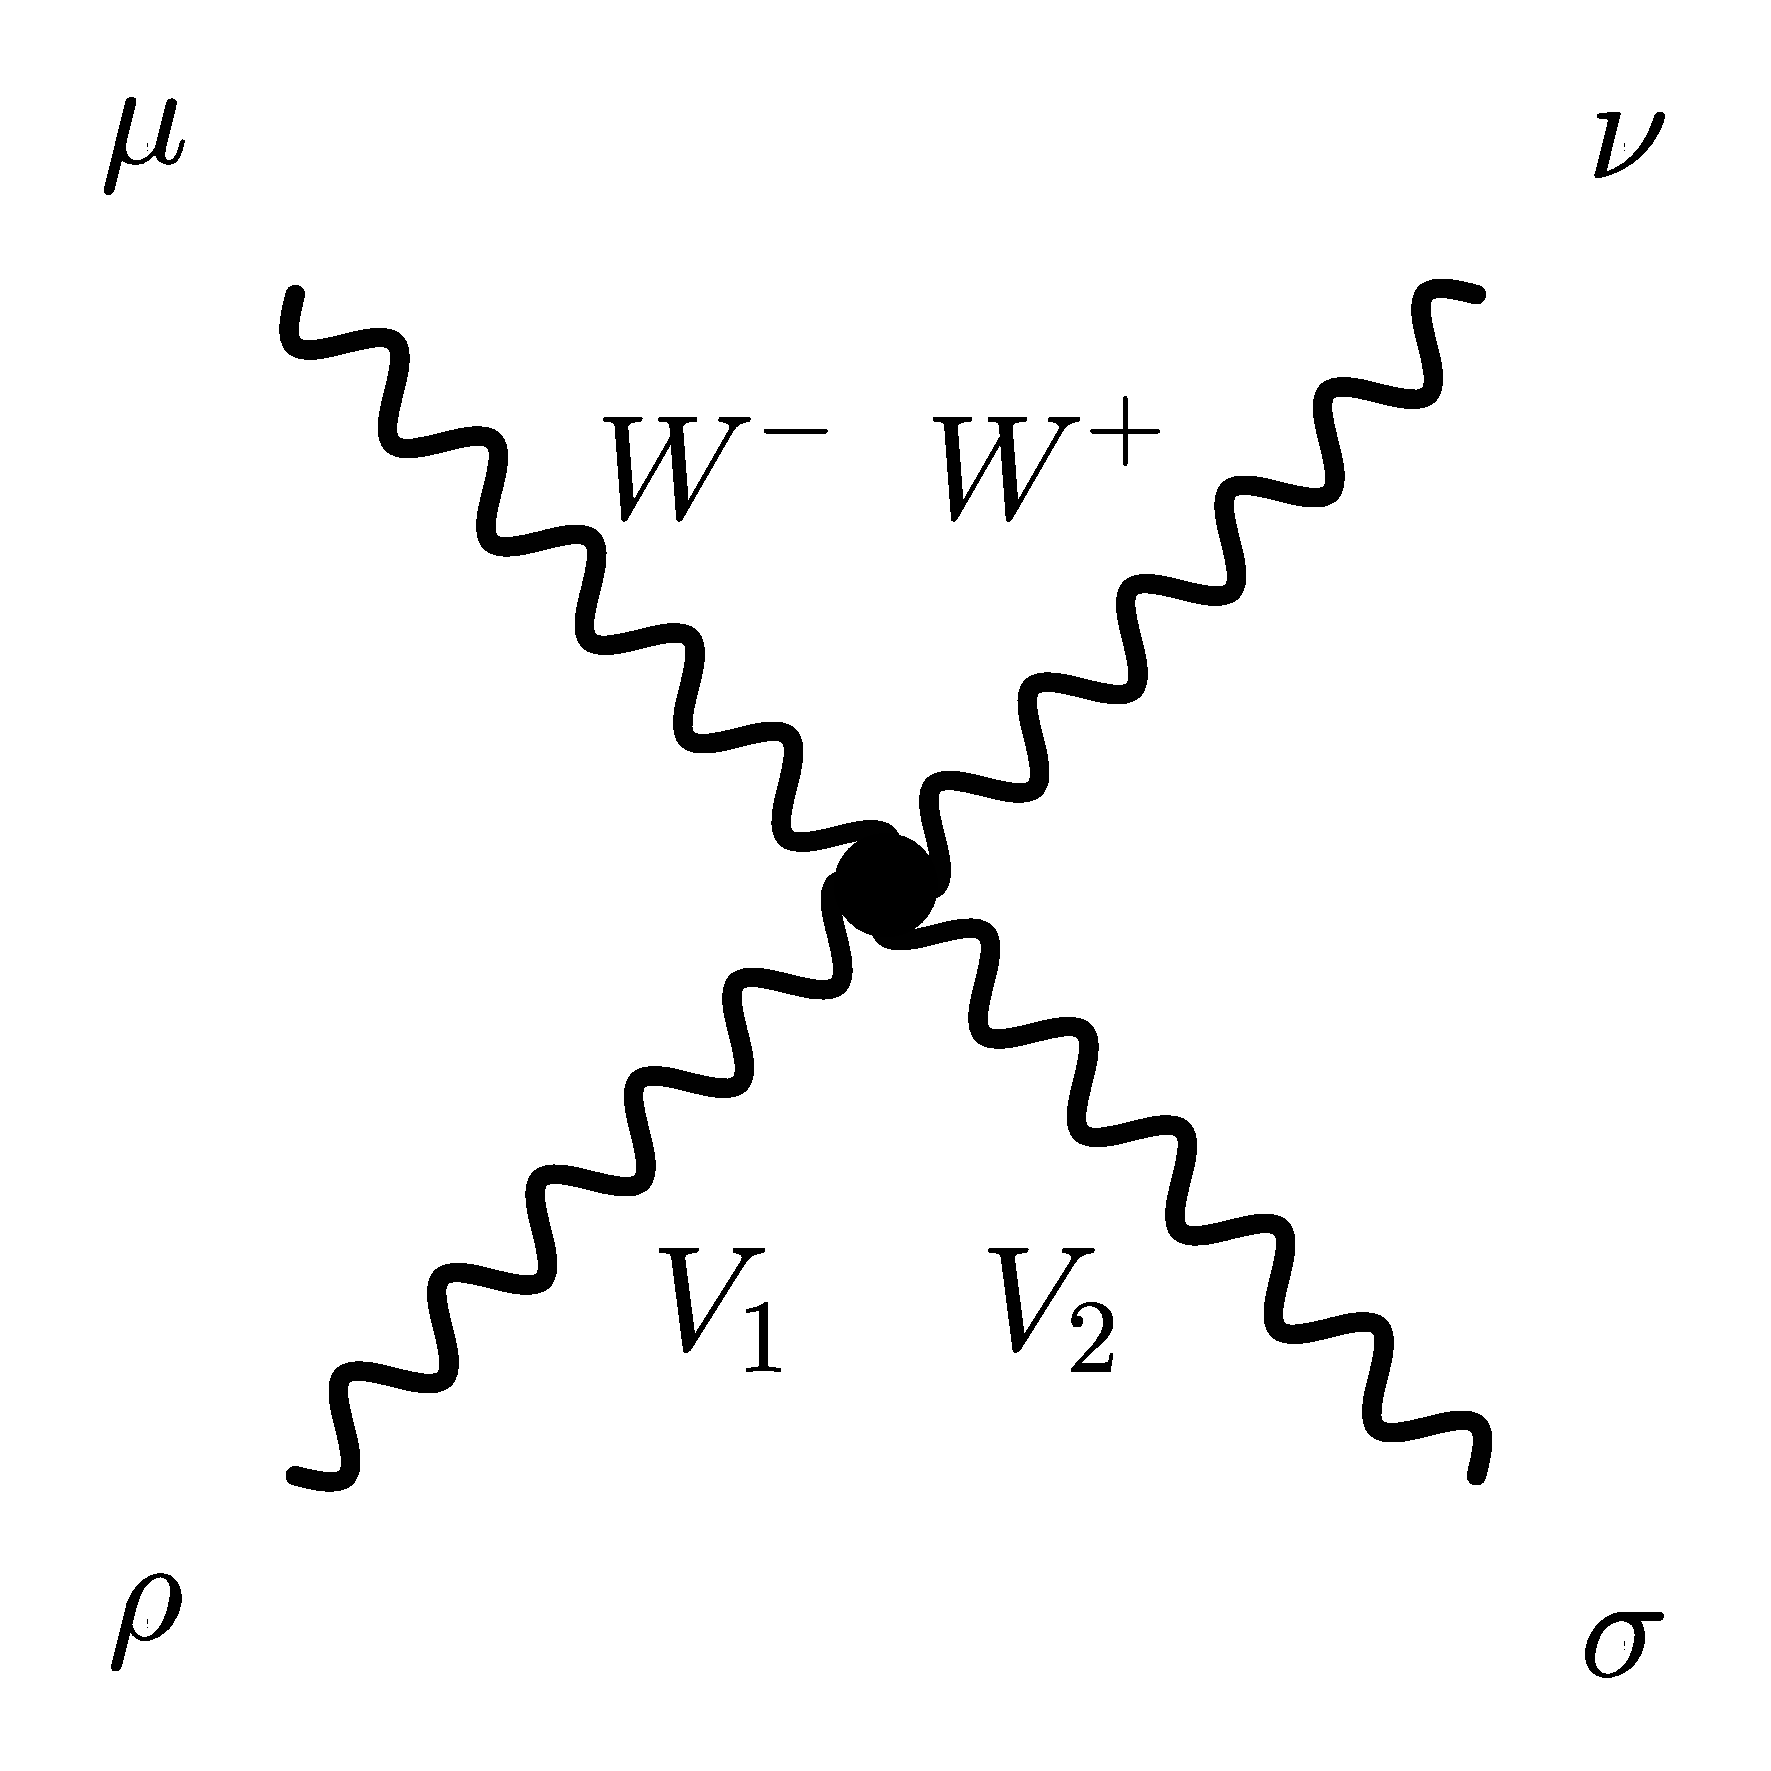
\includegraphics[width=3cm]{Images/FeynmanRules/WWVV_vertex.pdf}}} & = i \frac{e^2}{\sin^2 \theta_W} \left(g^{\mu \sigma} g^{\nu \rho} + g^{\mu \rho} g^{\nu \sigma} - 2 g^{\mu \nu} g^{\rho \sigma}  \right) \times \prod_{i=1}^2 \begin{cases} - \sin \theta_W  \quad &\text{if } V_i = \gamma \\ \cos \theta_W \quad & \text{if } V_i = Z \end{cases} \\
\vcenter{\hbox{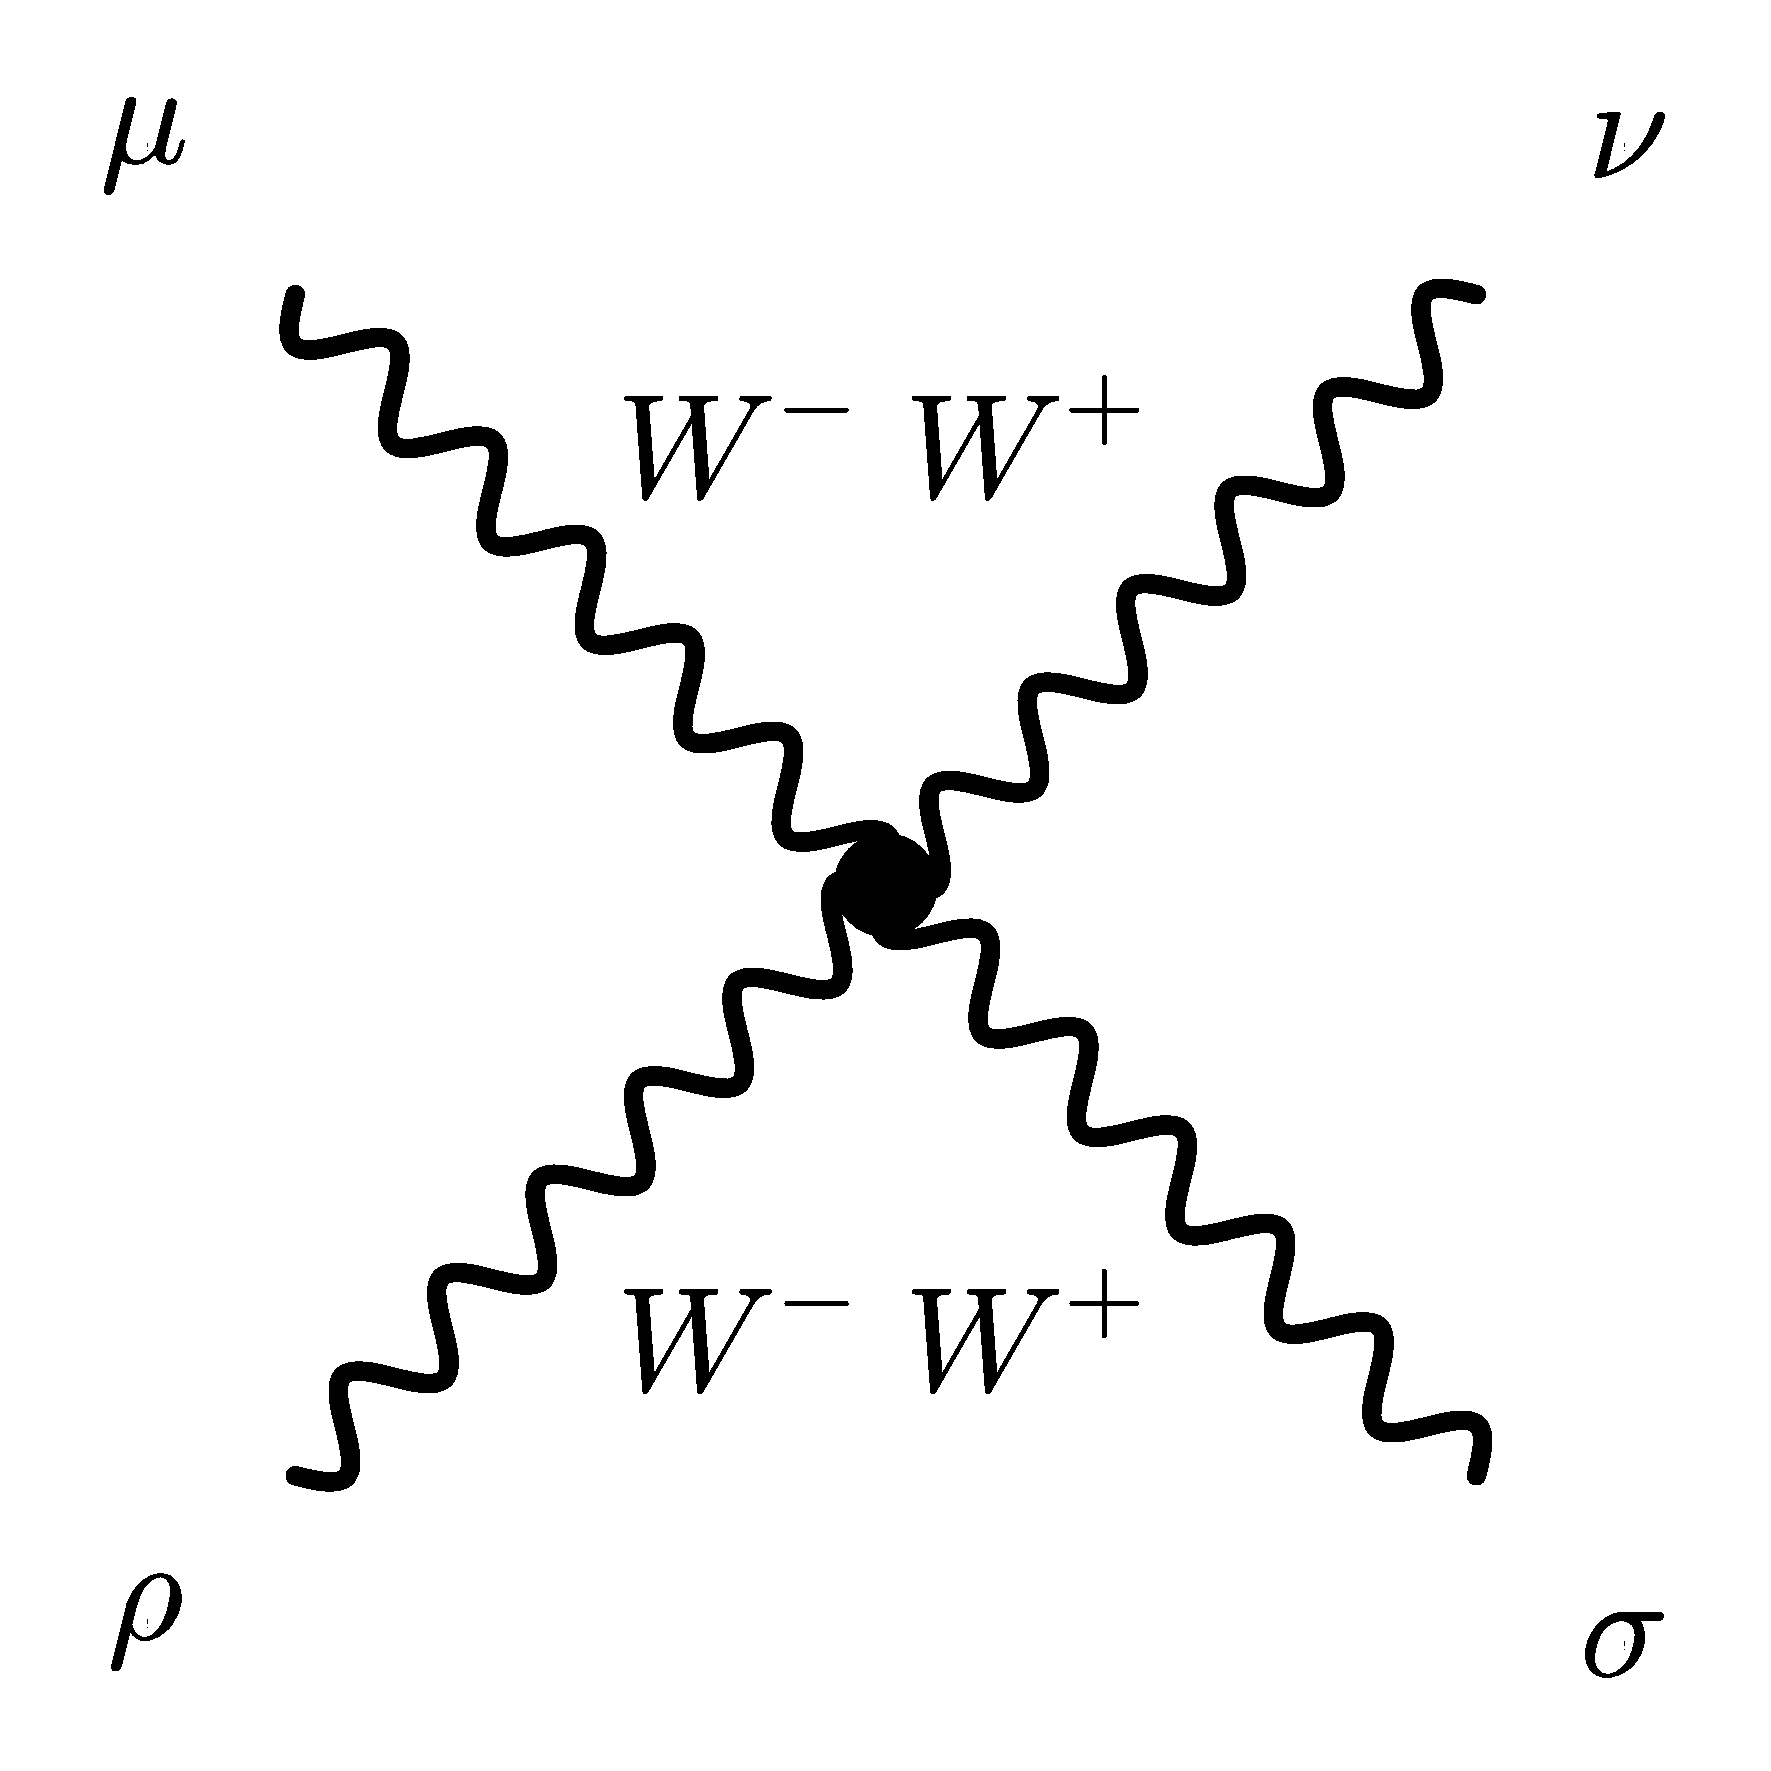
\includegraphics[width=3cm]{Images/FeynmanRules/WWWW_vertex.pdf}}} & = i \frac{e^2}{\sin^2 \theta_W} \left(2 g^{\mu \rho} g^{\nu \sigma} - g^{\mu \nu} g^{\rho \sigma} - g^{\mu \sigma} g^{\nu \rho} \right)
\end{alignat*}

\textbf{Higgs Interactions:}
\begin{alignat*}{3}
&\vcenter{\hbox{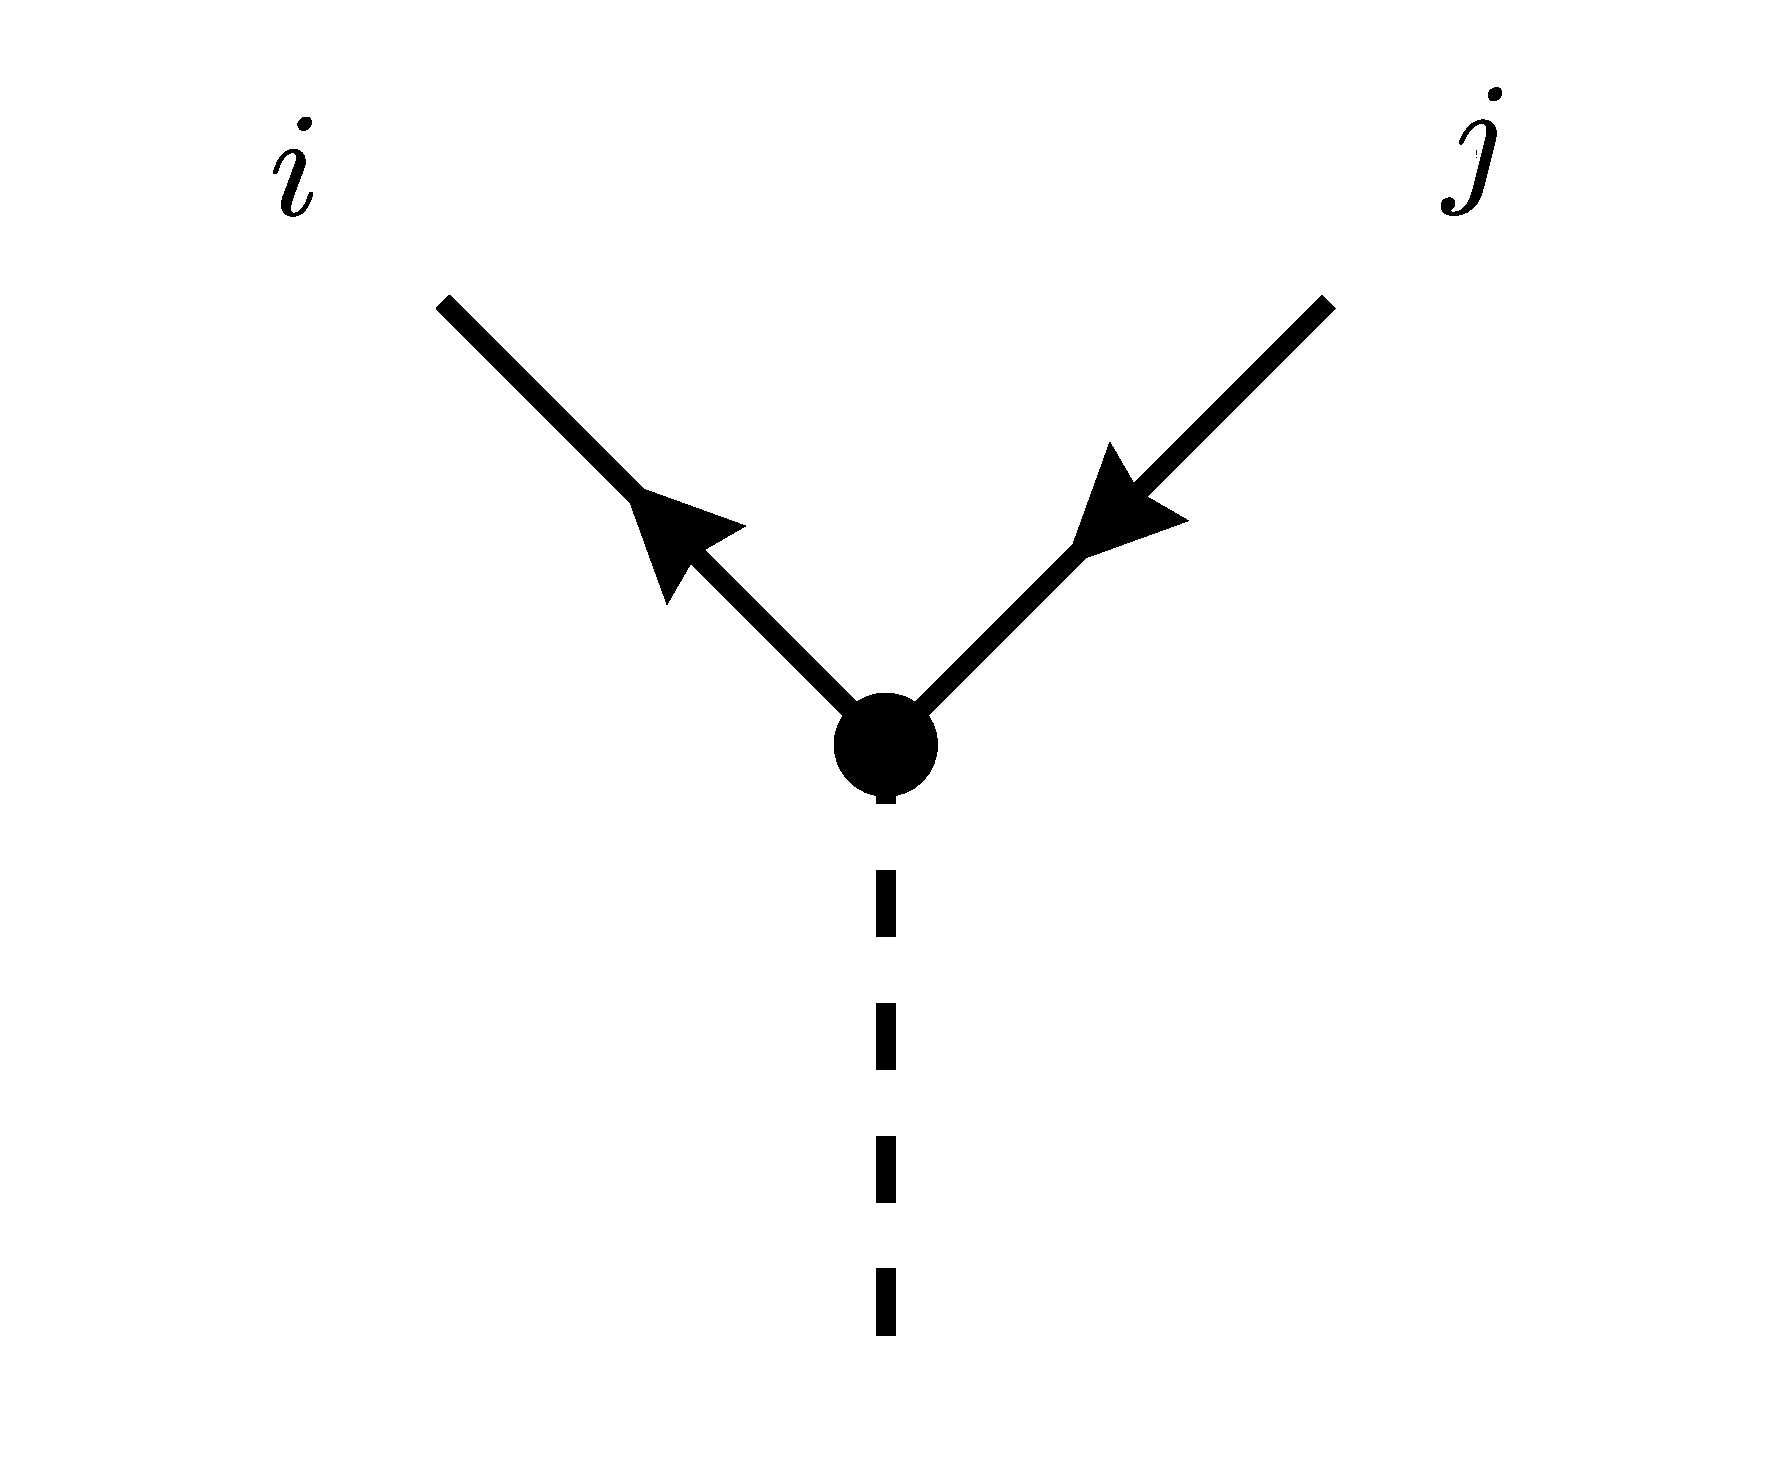
\includegraphics[width=3cm]{Images/FeynmanRules/Higgs_fermion_vertex.pdf}}} = -i \frac{m_q}{v} \delta_{ij} \quad
&&\vcenter{\hbox{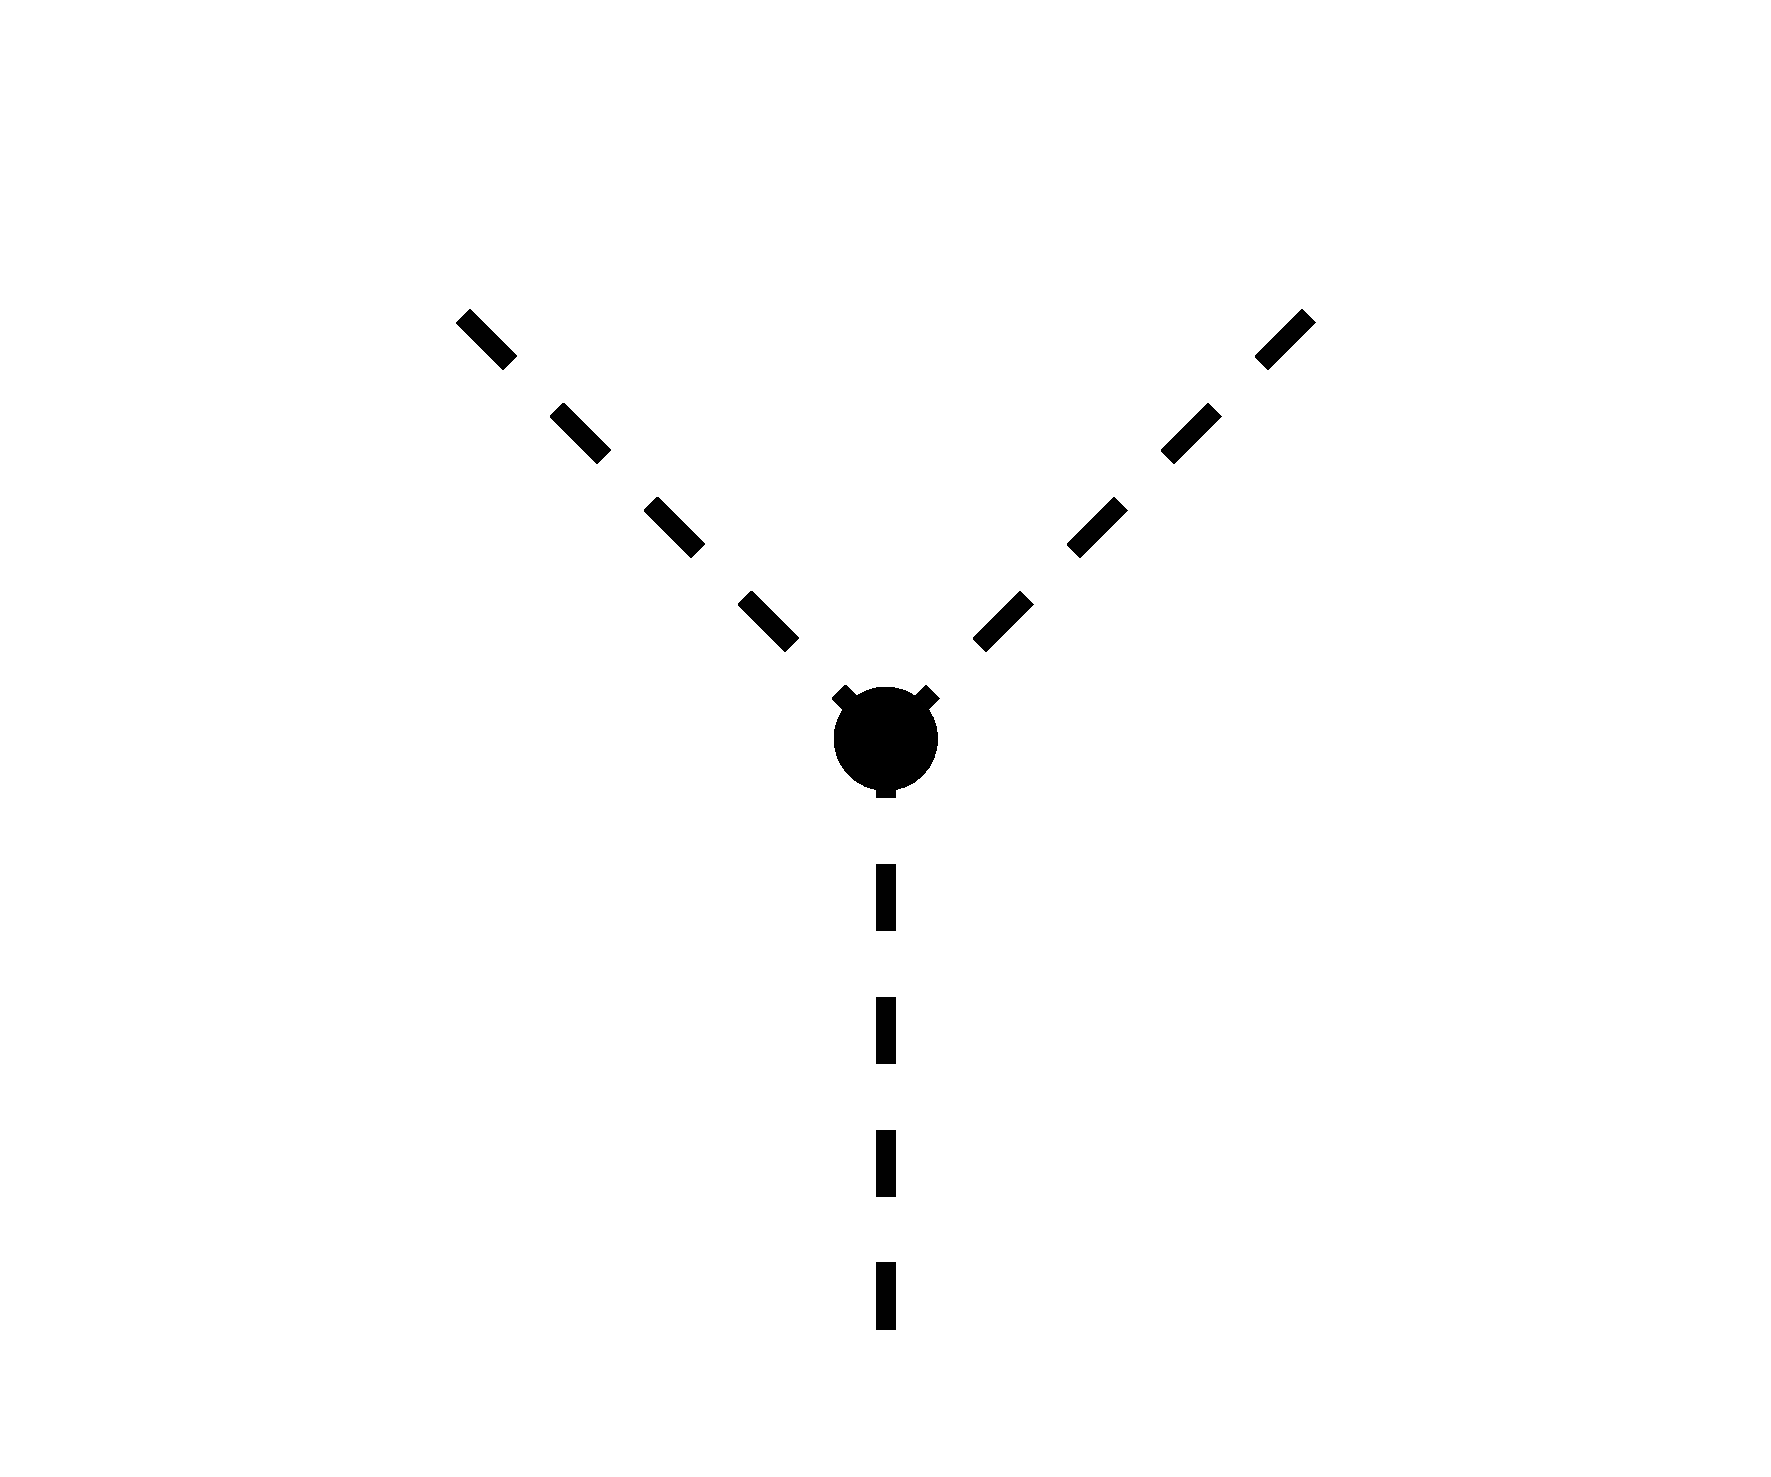
\includegraphics[width=3cm]{Images/FeynmanRules/triple_Higgs_vertex.pdf}}} = - i \frac{3 m_H^2}{v} \\
%
&\vcenter{\hbox{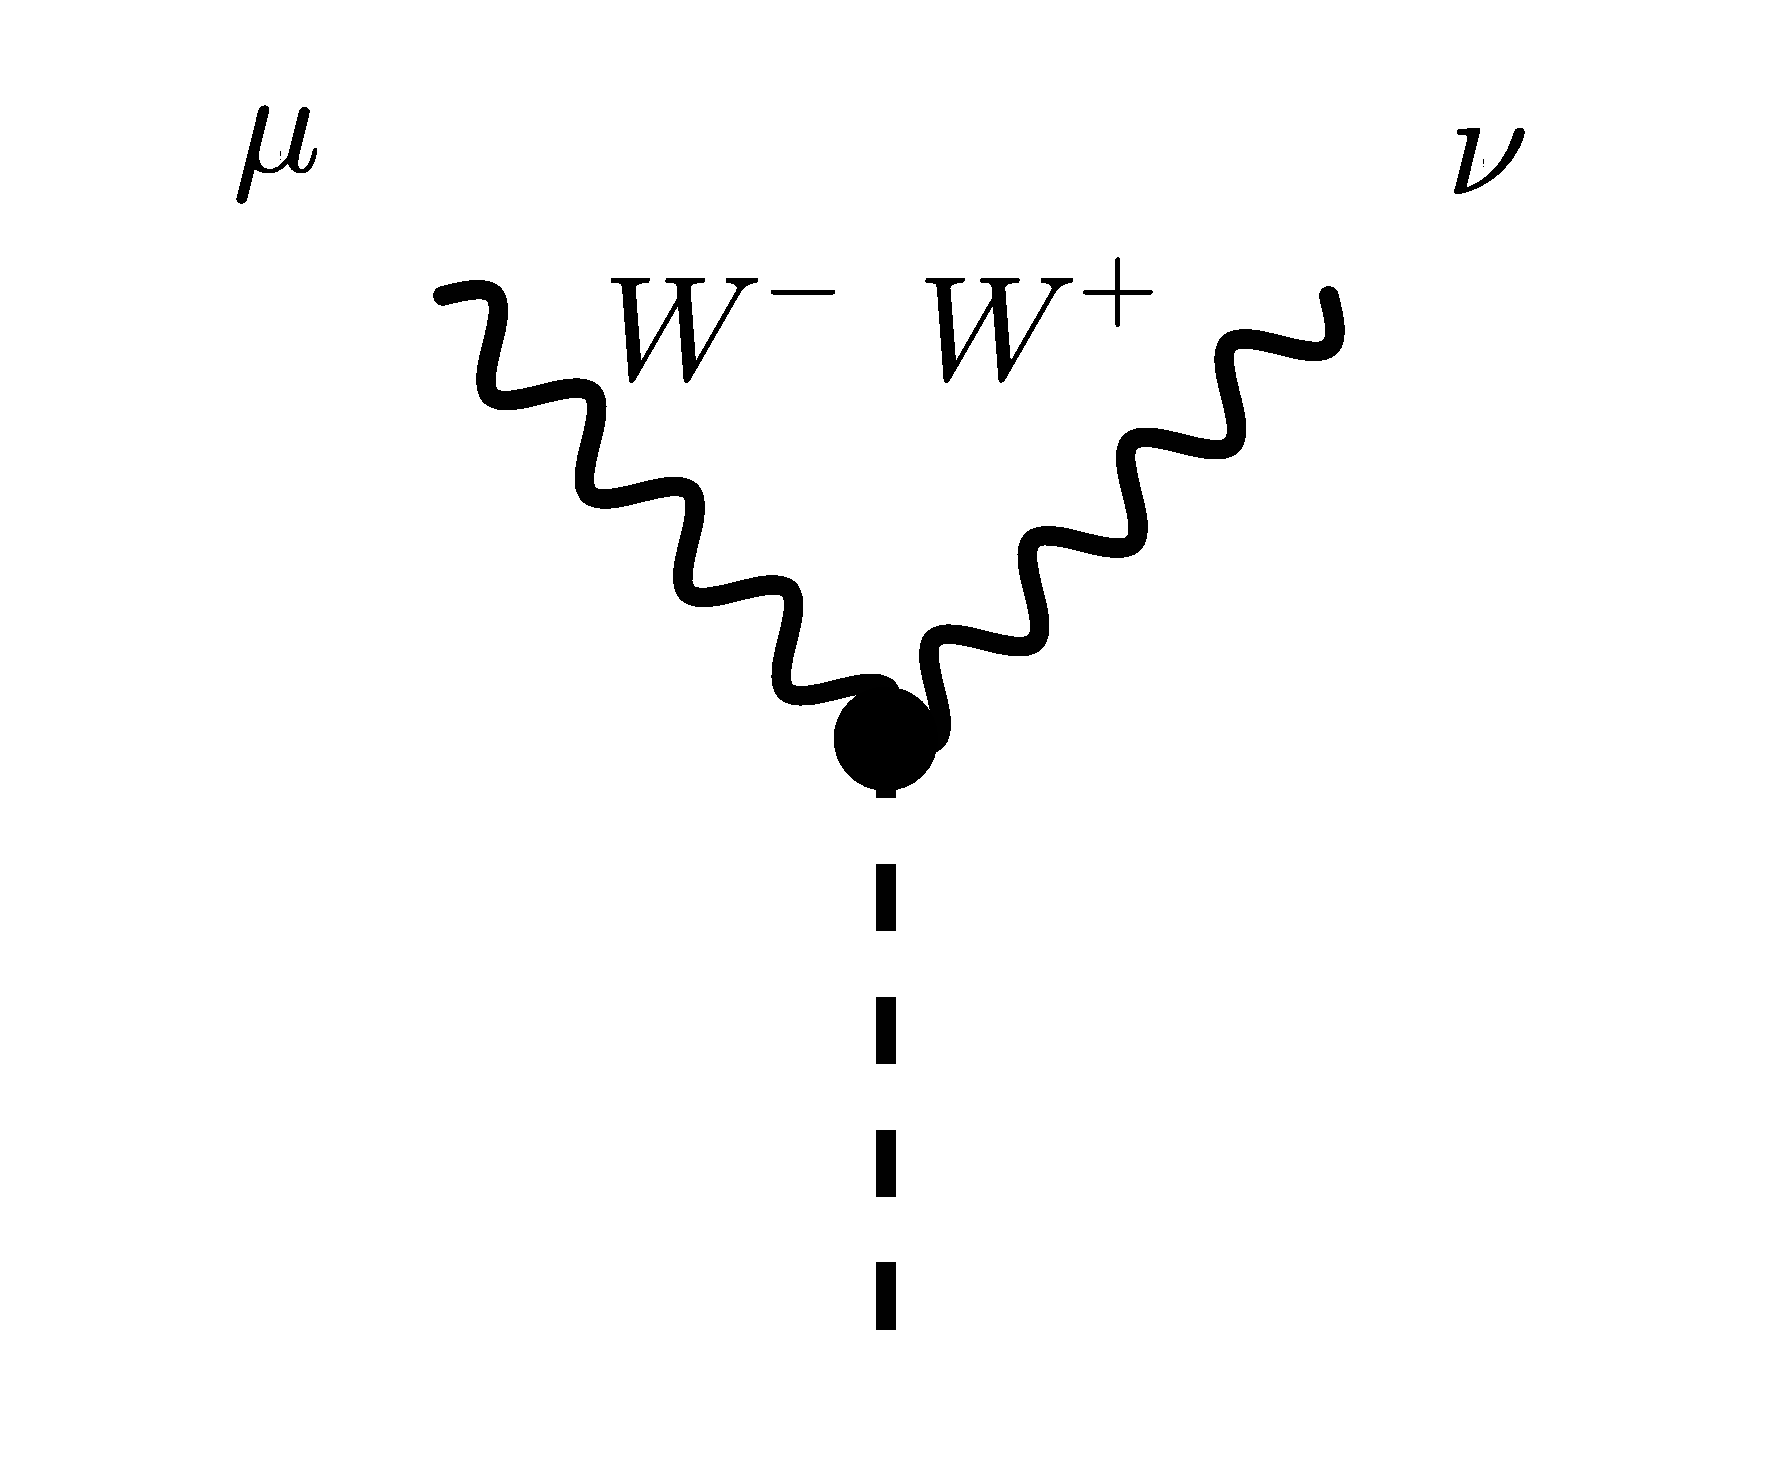
\includegraphics[width=3cm]{Images/FeynmanRules/WWH_vertex.pdf}}} = i \frac{e}{\sin \theta_W} m_W g^{\mu \nu} \quad
&&\vcenter{\hbox{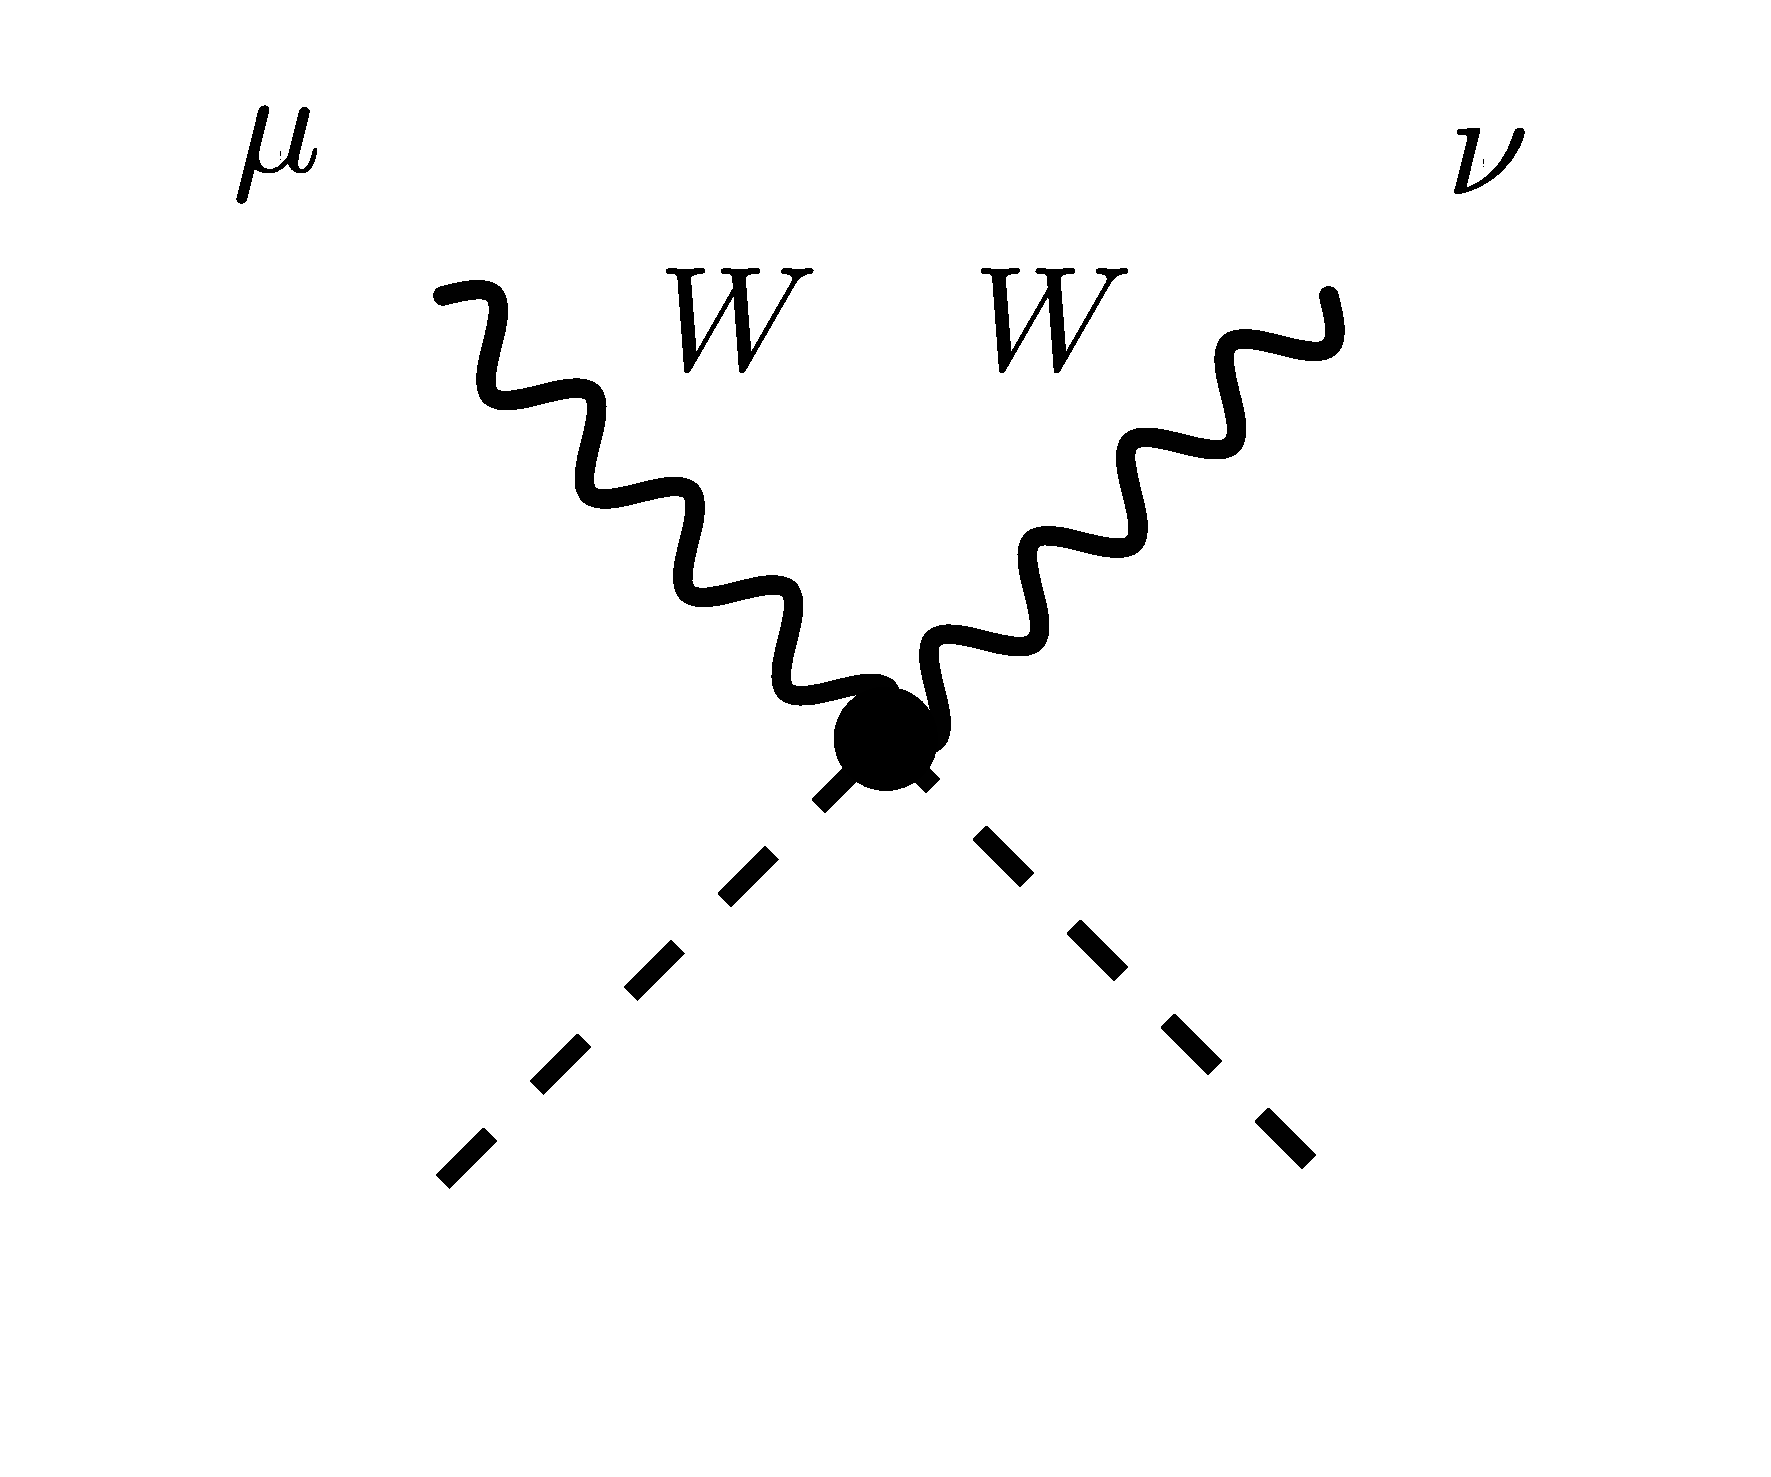
\includegraphics[width=3cm]{Images/FeynmanRules/WWHH_vertex.pdf}}} = i \frac{e^2}{2\sin^2 \theta_W }  g^{\mu \nu} \\
%
&\vcenter{\hbox{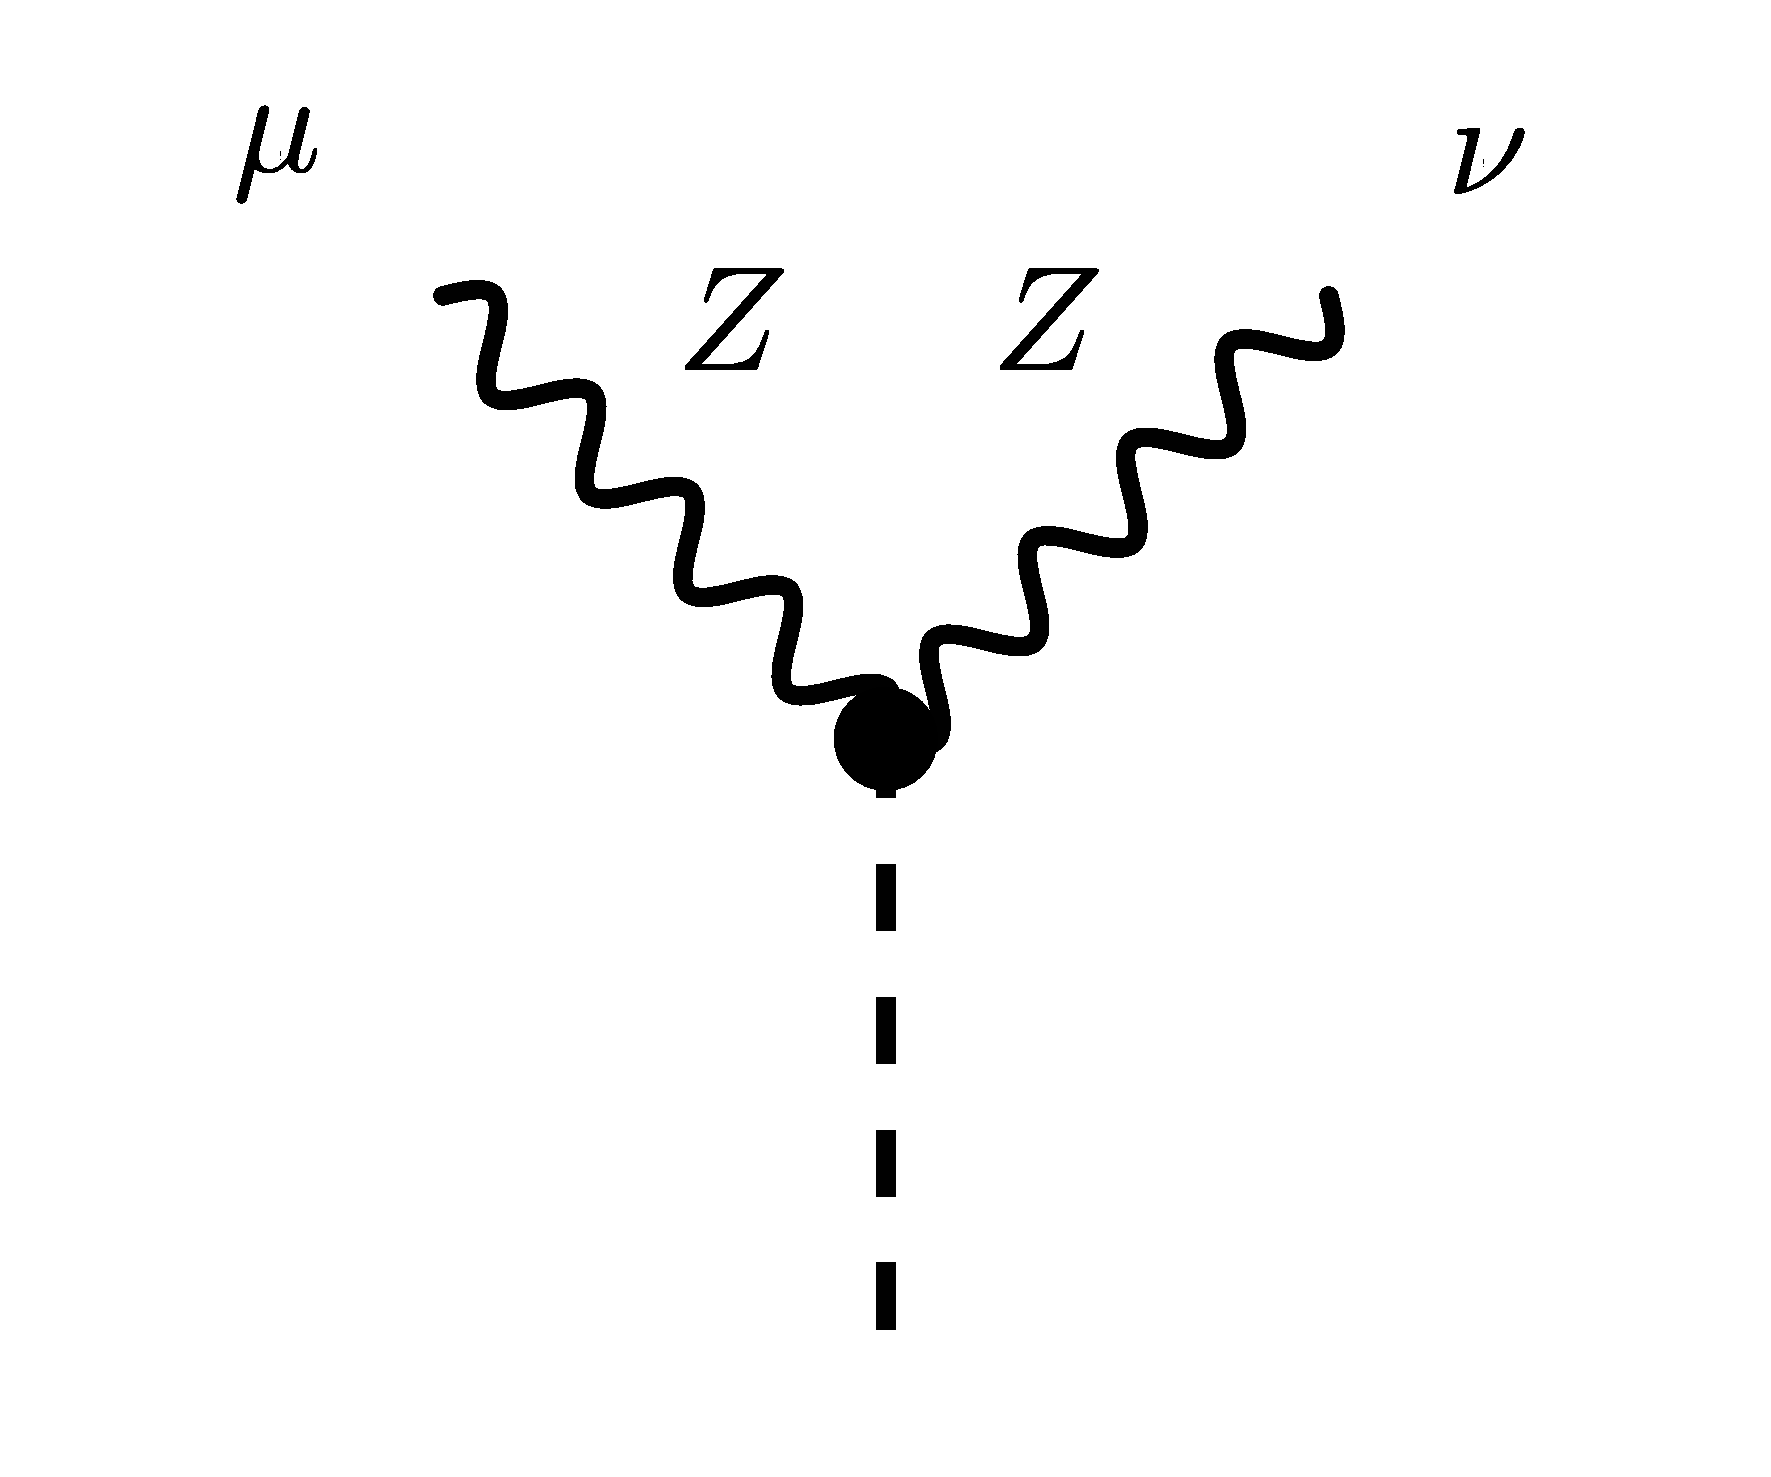
\includegraphics[width=3cm]{Images/FeynmanRules/ZZH_vertex.pdf}}} = i \frac{e}{\sin \theta_W \cos \theta_W} m_Z g^{\mu \nu} \quad
&&\vcenter{\hbox{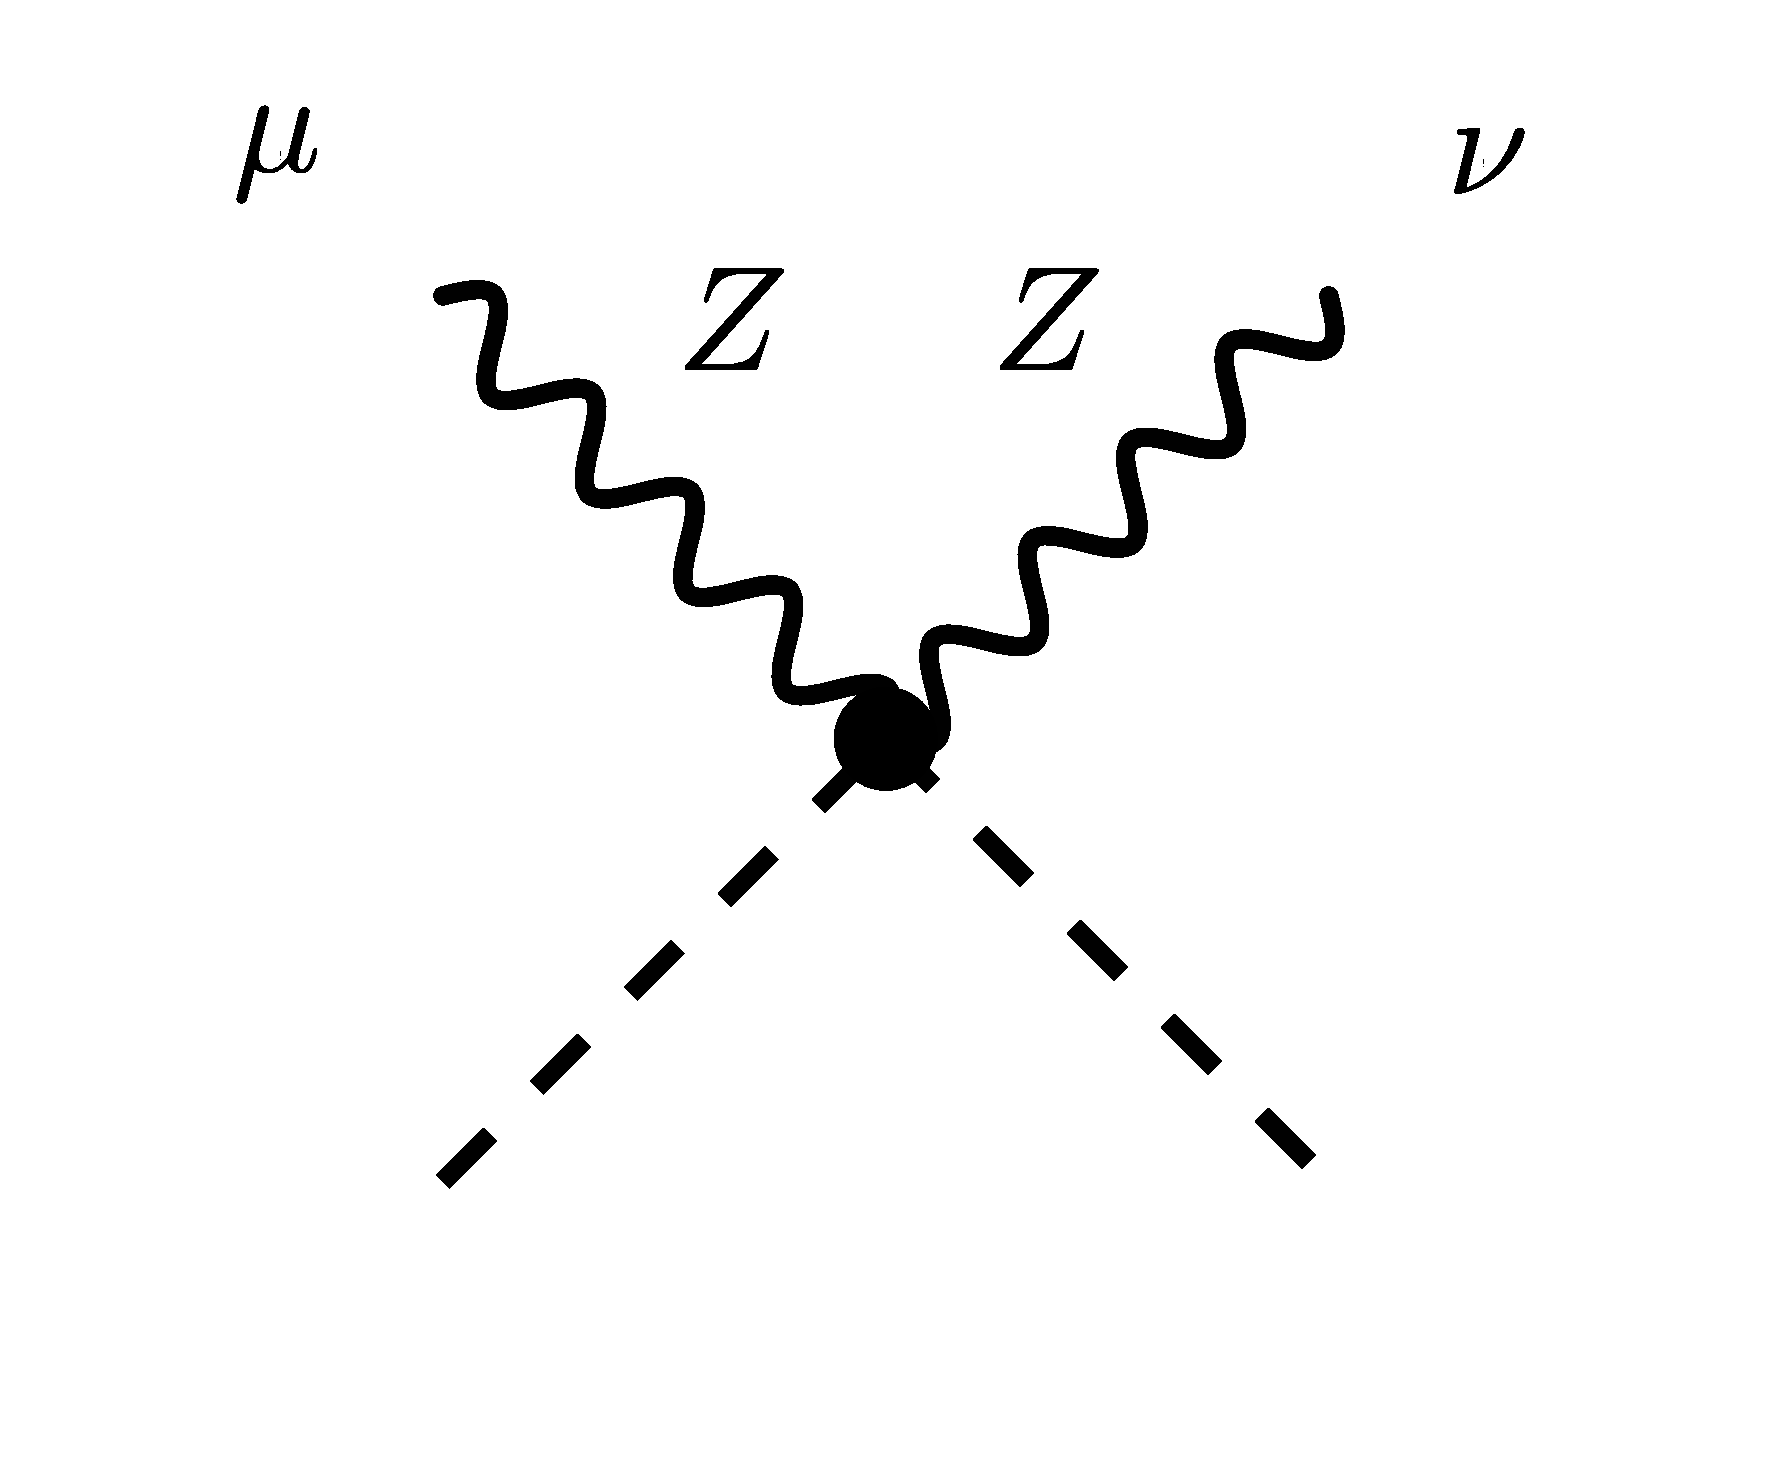
\includegraphics[width=3cm]{Images/FeynmanRules/ZZHH_vertex.pdf}}} = i \frac{e^2}{2\sin^2 \theta_W \cos^2 \theta_W}  g^{\mu \nu} \\
%
&\vcenter{\hbox{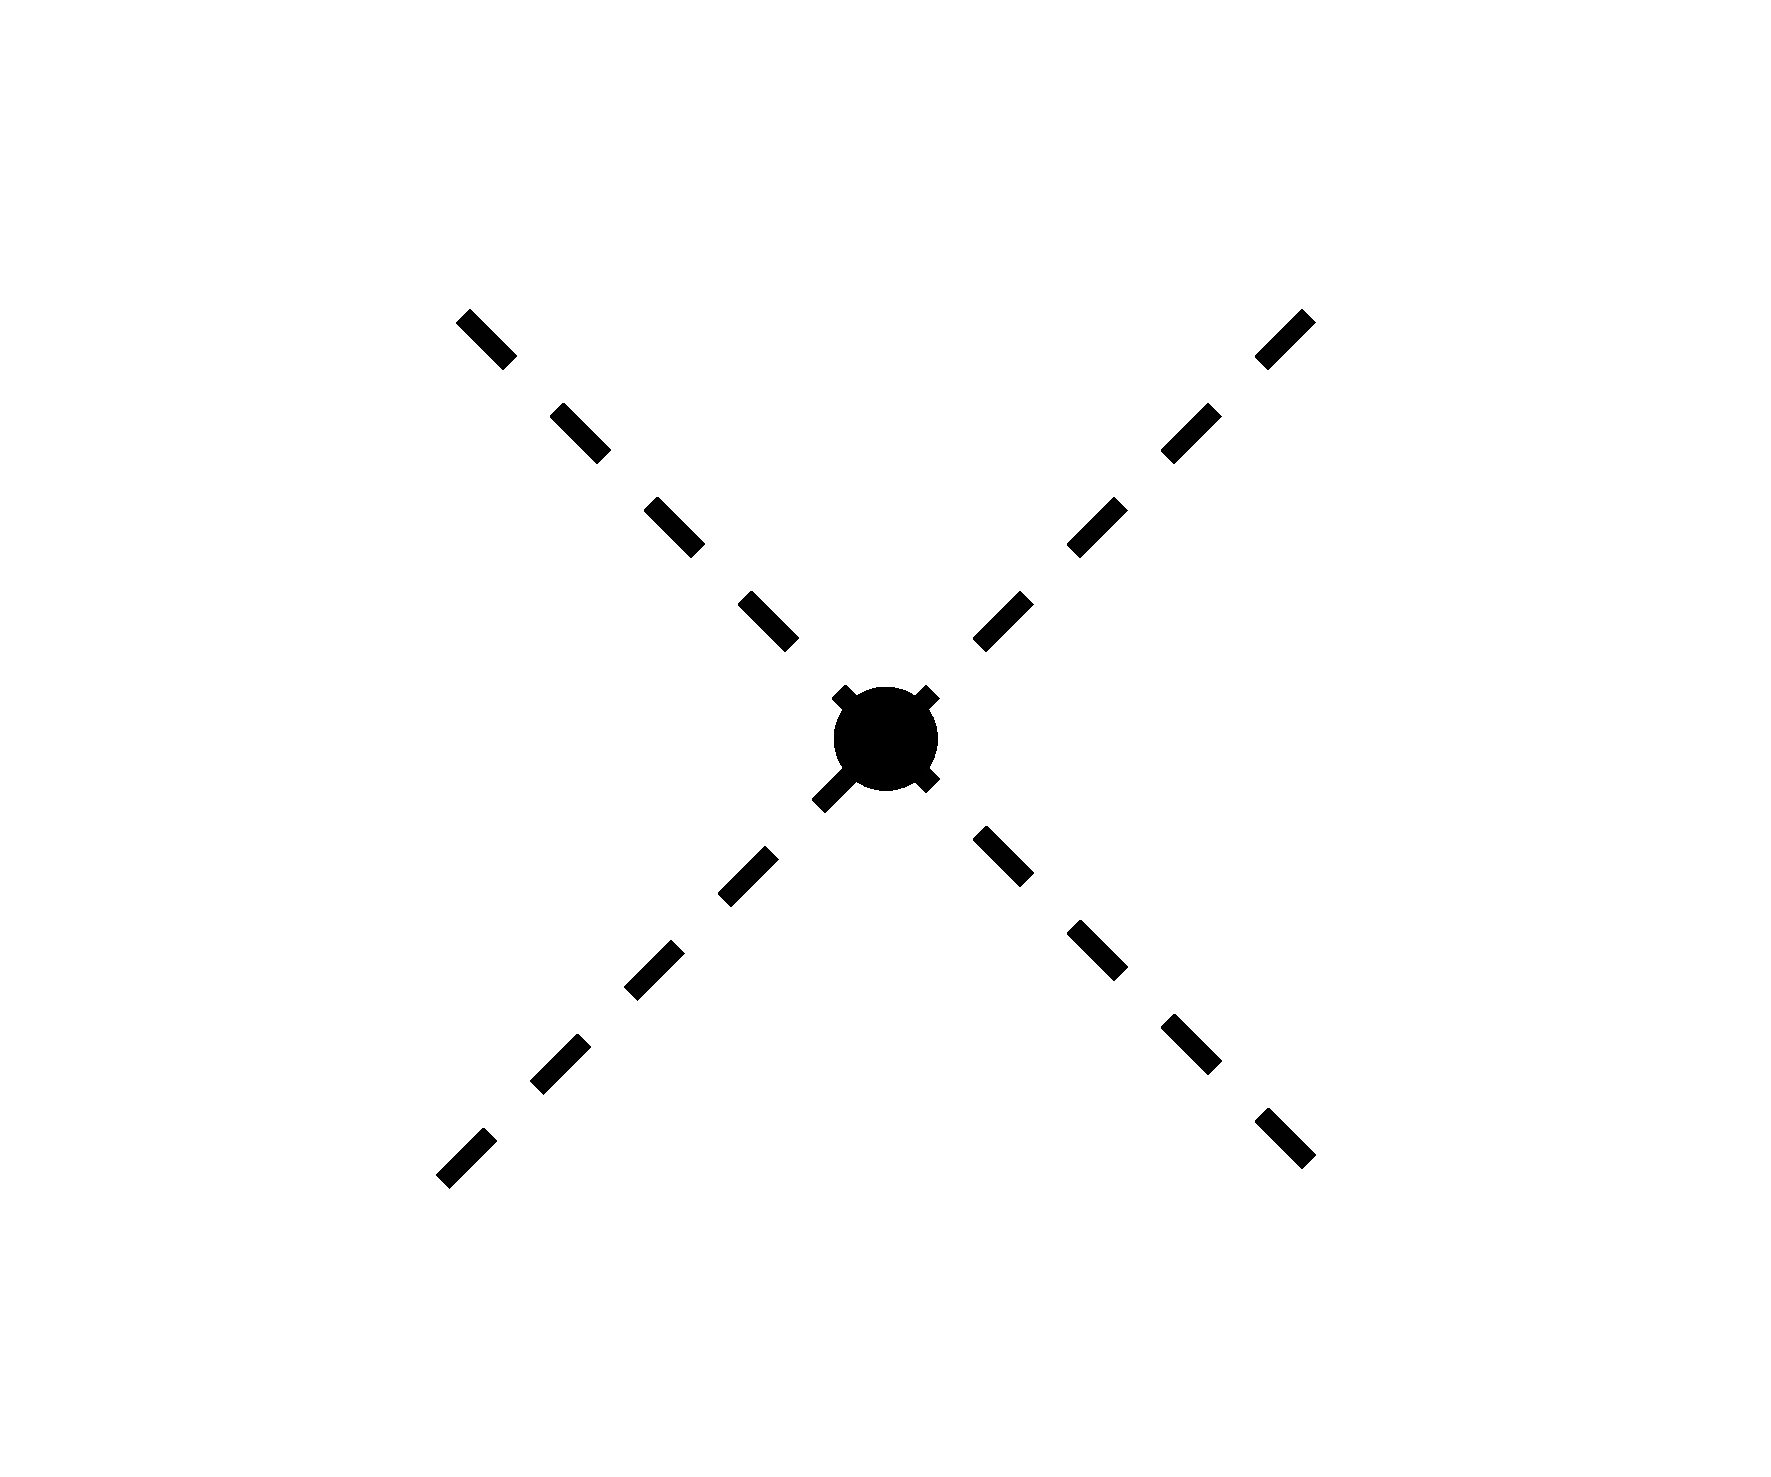
\includegraphics[width=3cm]{Images/FeynmanRules/quadruple_Higgs_vertex.pdf}}} = - i \frac{ 3 m_H^2}{v^2}
\end{alignat*}